\documentclass[twoside]{book}

% Packages required by doxygen
\usepackage{fixltx2e}
\usepackage{calc}
\usepackage{doxygen}
\usepackage[export]{adjustbox} % also loads graphicx
\usepackage{graphicx}
\usepackage[utf8]{inputenc}
\usepackage{makeidx}
\usepackage{multicol}
\usepackage{multirow}
\PassOptionsToPackage{warn}{textcomp}
\usepackage{textcomp}
\usepackage[nointegrals]{wasysym}
\usepackage[table]{xcolor}

% Font selection
\usepackage[T1]{fontenc}
\usepackage[scaled=.90]{helvet}
\usepackage{courier}
\usepackage{amssymb}
\usepackage{sectsty}
\renewcommand{\familydefault}{\sfdefault}
\allsectionsfont{%
  \fontseries{bc}\selectfont%
  \color{darkgray}%
}
\renewcommand{\DoxyLabelFont}{%
  \fontseries{bc}\selectfont%
  \color{darkgray}%
}
\newcommand{\+}{\discretionary{\mbox{\scriptsize$\hookleftarrow$}}{}{}}

% Page & text layout
\usepackage{geometry}
\geometry{%
  a4paper,%
  top=2.5cm,%
  bottom=2.5cm,%
  left=2.5cm,%
  right=2.5cm%
}
\tolerance=750
\hfuzz=15pt
\hbadness=750
\setlength{\emergencystretch}{15pt}
\setlength{\parindent}{0cm}
\setlength{\parskip}{3ex plus 2ex minus 2ex}
\makeatletter
\renewcommand{\paragraph}{%
  \@startsection{paragraph}{4}{0ex}{-1.0ex}{1.0ex}{%
    \normalfont\normalsize\bfseries\SS@parafont%
  }%
}
\renewcommand{\subparagraph}{%
  \@startsection{subparagraph}{5}{0ex}{-1.0ex}{1.0ex}{%
    \normalfont\normalsize\bfseries\SS@subparafont%
  }%
}
\makeatother

% Headers & footers
\usepackage{fancyhdr}
\pagestyle{fancyplain}
\fancyhead[LE]{\fancyplain{}{\bfseries\thepage}}
\fancyhead[CE]{\fancyplain{}{}}
\fancyhead[RE]{\fancyplain{}{\bfseries\leftmark}}
\fancyhead[LO]{\fancyplain{}{\bfseries\rightmark}}
\fancyhead[CO]{\fancyplain{}{}}
\fancyhead[RO]{\fancyplain{}{\bfseries\thepage}}
\fancyfoot[LE]{\fancyplain{}{}}
\fancyfoot[CE]{\fancyplain{}{}}
\fancyfoot[RE]{\fancyplain{}{\bfseries\scriptsize Generated by Doxygen }}
\fancyfoot[LO]{\fancyplain{}{\bfseries\scriptsize Generated by Doxygen }}
\fancyfoot[CO]{\fancyplain{}{}}
\fancyfoot[RO]{\fancyplain{}{}}
\renewcommand{\footrulewidth}{0.4pt}
\renewcommand{\chaptermark}[1]{%
  \markboth{#1}{}%
}
\renewcommand{\sectionmark}[1]{%
  \markright{\thesection\ #1}%
}

% Indices & bibliography
\usepackage{natbib}
\usepackage[titles]{tocloft}
\setcounter{tocdepth}{3}
\setcounter{secnumdepth}{5}
\makeindex

% Hyperlinks (required, but should be loaded last)
\usepackage{ifpdf}
\ifpdf
  \usepackage[pdftex,pagebackref=true]{hyperref}
\else
  \usepackage[ps2pdf,pagebackref=true]{hyperref}
\fi
\hypersetup{%
  colorlinks=true,%
  linkcolor=blue,%
  citecolor=blue,%
  unicode%
}

% Custom commands
\newcommand{\clearemptydoublepage}{%
  \newpage{\pagestyle{empty}\cleardoublepage}%
}

\usepackage{caption}
\captionsetup{labelsep=space,justification=centering,font={bf},singlelinecheck=off,skip=4pt,position=top}

%===== C O N T E N T S =====

\begin{document}

% Titlepage & ToC
\hypersetup{pageanchor=false,
             bookmarksnumbered=true,
             pdfencoding=unicode
            }
\pagenumbering{alph}
\begin{titlepage}
\vspace*{7cm}
\begin{center}%
{\Large Modules for recurent neural network \\[1ex]\large 0.\+1 }\\
\vspace*{1cm}
{\large Generated by Doxygen 1.8.13}\\
\end{center}
\end{titlepage}
\clearemptydoublepage
\pagenumbering{roman}
\tableofcontents
\clearemptydoublepage
\pagenumbering{arabic}
\hypersetup{pageanchor=true}

%--- Begin generated contents ---
\chapter{Hierarchical Index}
\section{Class Hierarchy}
This inheritance list is sorted roughly, but not completely, alphabetically\+:\begin{DoxyCompactList}
\item list\begin{DoxyCompactList}
\item \contentsline{section}{modules.\+Input\+Container}{\pageref{classmodules_1_1_input_container}}{}
\end{DoxyCompactList}
\item \contentsline{section}{modules.\+Module}{\pageref{classmodules_1_1_module}}{}
\begin{DoxyCompactList}
\item \contentsline{section}{modules.\+Abstract\+Composed\+Module}{\pageref{classmodules_1_1_abstract_composed_module}}{}
\begin{DoxyCompactList}
\item \contentsline{section}{modules.\+Composed\+Module}{\pageref{classmodules_1_1_composed_module}}{}
\begin{DoxyCompactList}
\item \contentsline{section}{modules.\+Convolutional\+Layer\+Module}{\pageref{classmodules_1_1_convolutional_layer_module}}{}
\item \contentsline{section}{modules.\+Fully\+Connected\+Layer\+Module}{\pageref{classmodules_1_1_fully_connected_layer_module}}{}
\end{DoxyCompactList}
\item \contentsline{section}{modules.\+Time\+Composed\+Module}{\pageref{classmodules_1_1_time_composed_module}}{}
\begin{DoxyCompactList}
\item \contentsline{section}{modules.\+Time\+Convolutional\+Layer\+Module}{\pageref{classmodules_1_1_time_convolutional_layer_module}}{}
\end{DoxyCompactList}
\end{DoxyCompactList}
\item \contentsline{section}{modules.\+Operation\+Module}{\pageref{classmodules_1_1_operation_module}}{}
\begin{DoxyCompactList}
\item \contentsline{section}{modules.\+Activation\+Module}{\pageref{classmodules_1_1_activation_module}}{}
\item \contentsline{section}{modules.\+Add\+Module}{\pageref{classmodules_1_1_add_module}}{}
\item \contentsline{section}{modules.\+Batch\+Accuracy\+Module}{\pageref{classmodules_1_1_batch_accuracy_module}}{}
\item \contentsline{section}{modules.\+Composed\+Module}{\pageref{classmodules_1_1_composed_module}}{}
\item \contentsline{section}{modules.\+Error\+Module}{\pageref{classmodules_1_1_error_module}}{}
\item \contentsline{section}{modules.\+Flatten\+Module}{\pageref{classmodules_1_1_flatten_module}}{}
\item \contentsline{section}{modules.\+Max\+Pooling\+Module}{\pageref{classmodules_1_1_max_pooling_module}}{}
\item \contentsline{section}{modules.\+Optimizer\+Module}{\pageref{classmodules_1_1_optimizer_module}}{}
\item \contentsline{section}{modules.\+Time\+Operation\+Module}{\pageref{classmodules_1_1_time_operation_module}}{}
\begin{DoxyCompactList}
\item \contentsline{section}{modules.\+Fake\+Module}{\pageref{classmodules_1_1_fake_module}}{}
\item \contentsline{section}{modules.\+Time\+Add\+Module}{\pageref{classmodules_1_1_time_add_module}}{}
\item \contentsline{section}{modules.\+Time\+Composed\+Module}{\pageref{classmodules_1_1_time_composed_module}}{}
\end{DoxyCompactList}
\item \contentsline{section}{modules.\+Variable\+Module}{\pageref{classmodules_1_1_variable_module}}{}
\begin{DoxyCompactList}
\item \contentsline{section}{modules.\+Bias\+Module}{\pageref{classmodules_1_1_bias_module}}{}
\item \contentsline{section}{modules.\+Conv2\+D\+Module}{\pageref{classmodules_1_1_conv2_d_module}}{}
\item \contentsline{section}{modules.\+Conv2\+D\+Transpose\+Module}{\pageref{classmodules_1_1_conv2_d_transpose_module}}{}
\item \contentsline{section}{modules.\+Fully\+Connected\+Module}{\pageref{classmodules_1_1_fully_connected_module}}{}
\end{DoxyCompactList}
\end{DoxyCompactList}
\item \contentsline{section}{modules.\+Placeholder\+Module}{\pageref{classmodules_1_1_placeholder_module}}{}
\begin{DoxyCompactList}
\item \contentsline{section}{modules.\+Constant\+Placeholder\+Module}{\pageref{classmodules_1_1_constant_placeholder_module}}{}
\item \contentsline{section}{modules.\+Time\+Varying\+Placeholder\+Module}{\pageref{classmodules_1_1_time_varying_placeholder_module}}{}
\end{DoxyCompactList}
\end{DoxyCompactList}
\end{DoxyCompactList}

\chapter{Class Index}
\section{Class List}
Here are the classes, structs, unions and interfaces with brief descriptions\+:\begin{DoxyCompactList}
\item\contentsline{section}{\hyperlink{classmodules_1_1_abstract_composed_module}{modules.\+Abstract\+Composed\+Module} }{\pageref{classmodules_1_1_abstract_composed_module}}{}
\item\contentsline{section}{\hyperlink{classmodules_1_1_activation_module}{modules.\+Activation\+Module} \\*Apply an activation function on its input module }{\pageref{classmodules_1_1_activation_module}}{}
\item\contentsline{section}{\hyperlink{classmodules_1_1_add_module}{modules.\+Add\+Module} \\*This module computes the sum of all its input }{\pageref{classmodules_1_1_add_module}}{}
\item\contentsline{section}{\hyperlink{classmodules_1_1_batch_accuracy_module}{modules.\+Batch\+Accuracy\+Module} \\*\hyperlink{classmodules_1_1_module}{Module} to compute the classification accuracy }{\pageref{classmodules_1_1_batch_accuracy_module}}{}
\item\contentsline{section}{\hyperlink{classmodules_1_1_bias_module}{modules.\+Bias\+Module} \\*\hyperlink{classmodules_1_1_module}{Module} to create a bias, that can be added to an other tensor inputs modules of this module are not taken into account }{\pageref{classmodules_1_1_bias_module}}{}
\item\contentsline{section}{\hyperlink{classmodules_1_1_composed_module}{modules.\+Composed\+Module} \\*This class is an abstract class which allows when overwritten to create a module that is composed of other modules and does not accept recursions See the implementation of \hyperlink{classmodules_1_1_convolutional_layer_module}{Convolutional\+Layer\+Module} for more info }{\pageref{classmodules_1_1_composed_module}}{}
\item\contentsline{section}{\hyperlink{classmodules_1_1_constant_placeholder_module}{modules.\+Constant\+Placeholder\+Module} \\*\hyperlink{classmodules_1_1_module}{Module} to reserve a place to feed in data }{\pageref{classmodules_1_1_constant_placeholder_module}}{}
\item\contentsline{section}{\hyperlink{classmodules_1_1_conv2_d_module}{modules.\+Conv2\+D\+Module} \\*\hyperlink{classmodules_1_1_module}{Module} to perform a convolution }{\pageref{classmodules_1_1_conv2_d_module}}{}
\item\contentsline{section}{\hyperlink{classmodules_1_1_conv2_d_transpose_module}{modules.\+Conv2\+D\+Transpose\+Module} \\*\hyperlink{classmodules_1_1_module}{Module} to perform a deconvolution }{\pageref{classmodules_1_1_conv2_d_transpose_module}}{}
\item\contentsline{section}{\hyperlink{classmodules_1_1_convolutional_layer_module}{modules.\+Convolutional\+Layer\+Module} \\*This composed module performs a convolution and applies a bias and an activation function }{\pageref{classmodules_1_1_convolutional_layer_module}}{}
\item\contentsline{section}{\hyperlink{classmodules_1_1_error_module}{modules.\+Error\+Module} \\*\hyperlink{classmodules_1_1_module}{Module} to compute an error (or apply any tensorflow operation on two and only two tensors) }{\pageref{classmodules_1_1_error_module}}{}
\item\contentsline{section}{\hyperlink{classmodules_1_1_fake_module}{modules.\+Fake\+Module} \\*For testing purpose only, does nothing }{\pageref{classmodules_1_1_fake_module}}{}
\item\contentsline{section}{\hyperlink{classmodules_1_1_flatten_module}{modules.\+Flatten\+Module} \\*\hyperlink{classmodules_1_1_module}{Module} to flatten the output of the input module }{\pageref{classmodules_1_1_flatten_module}}{}
\item\contentsline{section}{\hyperlink{classmodules_1_1_fully_connected_layer_module}{modules.\+Fully\+Connected\+Layer\+Module} \\*This composed module performs a full connection and applies a bias and an activation function }{\pageref{classmodules_1_1_fully_connected_layer_module}}{}
\item\contentsline{section}{\hyperlink{classmodules_1_1_fully_connected_module}{modules.\+Fully\+Connected\+Module} \\*\hyperlink{classmodules_1_1_module}{Module} to perform a matrix multiplication }{\pageref{classmodules_1_1_fully_connected_module}}{}
\item\contentsline{section}{\hyperlink{classmodules_1_1_input_container}{modules.\+Input\+Container} }{\pageref{classmodules_1_1_input_container}}{}
\item\contentsline{section}{\hyperlink{classmodules_1_1_max_pooling_module}{modules.\+Max\+Pooling\+Module} \\*\hyperlink{classmodules_1_1_module}{Module} to perform a maxpooling }{\pageref{classmodules_1_1_max_pooling_module}}{}
\item\contentsline{section}{\hyperlink{classmodules_1_1_module}{modules.\+Module} \\*Base class of a module }{\pageref{classmodules_1_1_module}}{}
\item\contentsline{section}{\hyperlink{classmodules_1_1_operation_module}{modules.\+Operation\+Module} \\*An operation module is a module that can perform an operation on the output of an other module in the same time slice }{\pageref{classmodules_1_1_operation_module}}{}
\item\contentsline{section}{\hyperlink{classmodules_1_1_optimizer_module}{modules.\+Optimizer\+Module} \\*\hyperlink{classmodules_1_1_module}{Module} to train a network }{\pageref{classmodules_1_1_optimizer_module}}{}
\item\contentsline{section}{\hyperlink{classmodules_1_1_placeholder_module}{modules.\+Placeholder\+Module} \\*A placeholder module is a module that takes no input }{\pageref{classmodules_1_1_placeholder_module}}{}
\item\contentsline{section}{\hyperlink{classmodules_1_1_time_add_module}{modules.\+Time\+Add\+Module} \\*This module computes the sum of all its input }{\pageref{classmodules_1_1_time_add_module}}{}
\item\contentsline{section}{\hyperlink{classmodules_1_1_time_composed_module}{modules.\+Time\+Composed\+Module} \\*This class is an abstract class which allows when overwritten to create a module that is composed of other modules and accept recursions See the implementation of \hyperlink{classmodules_1_1_convolutional_layer_module}{Convolutional\+Layer\+Module} for more info }{\pageref{classmodules_1_1_time_composed_module}}{}
\item\contentsline{section}{\hyperlink{classmodules_1_1_time_convolutional_layer_module}{modules.\+Time\+Convolutional\+Layer\+Module} \\*This composed module performs a convolution and applies a bias and an activation function }{\pageref{classmodules_1_1_time_convolutional_layer_module}}{}
\item\contentsline{section}{\hyperlink{classmodules_1_1_time_operation_module}{modules.\+Time\+Operation\+Module} \\*Same as an \hyperlink{classmodules_1_1_operation_module}{Operation\+Module} but this class allows to connect itself with the output of an other module in a different time slice }{\pageref{classmodules_1_1_time_operation_module}}{}
\item\contentsline{section}{\hyperlink{classmodules_1_1_time_varying_placeholder_module}{modules.\+Time\+Varying\+Placeholder\+Module} \\*\hyperlink{classmodules_1_1_module}{Module} to reserve a place to feed in data }{\pageref{classmodules_1_1_time_varying_placeholder_module}}{}
\item\contentsline{section}{\hyperlink{classmodules_1_1_variable_module}{modules.\+Variable\+Module} \\*This class allows a module to hold a tensorflow variable }{\pageref{classmodules_1_1_variable_module}}{}
\end{DoxyCompactList}

\chapter{Class Documentation}
\hypertarget{classmodules_1_1_abstract_composed_module}{}\section{modules.\+Abstract\+Composed\+Module Class Reference}
\label{classmodules_1_1_abstract_composed_module}\index{modules.\+Abstract\+Composed\+Module@{modules.\+Abstract\+Composed\+Module}}


Inheritance diagram for modules.\+Abstract\+Composed\+Module\+:\nopagebreak
\begin{figure}[H]
\begin{center}
\leavevmode
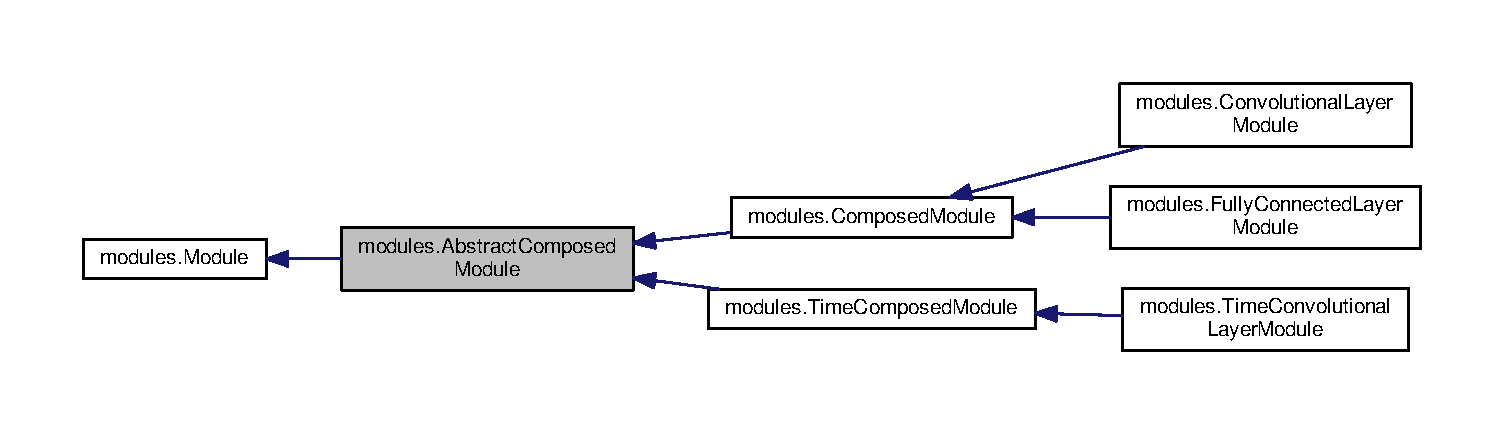
\includegraphics[width=350pt]{classmodules_1_1_abstract_composed_module__inherit__graph}
\end{center}
\end{figure}
\subsection*{Public Member Functions}
\begin{DoxyCompactItemize}
\item 
\mbox{\Hypertarget{classmodules_1_1_abstract_composed_module_a8571bf37cea3ff86c4a20cea449b0719}\label{classmodules_1_1_abstract_composed_module_a8571bf37cea3ff86c4a20cea449b0719}} 
def {\bfseries \+\_\+\+\_\+init\+\_\+\+\_\+} (self, args, kwargs)
\item 
\mbox{\Hypertarget{classmodules_1_1_abstract_composed_module_a8418c1a28b4bfab116ecbebf54d9fed9}\label{classmodules_1_1_abstract_composed_module_a8418c1a28b4bfab116ecbebf54d9fed9}} 
def {\bfseries create\+\_\+output} (self, t)
\item 
\mbox{\Hypertarget{classmodules_1_1_abstract_composed_module_aea4e1d5142ca898e92b82aa10e4aed88}\label{classmodules_1_1_abstract_composed_module_aea4e1d5142ca898e92b82aa10e4aed88}} 
def {\bfseries define\+\_\+inner\+\_\+modules} (self, args, kwargs)
\end{DoxyCompactItemize}
\subsection*{Public Attributes}
\begin{DoxyCompactItemize}
\item 
\mbox{\Hypertarget{classmodules_1_1_abstract_composed_module_a413abab6640553ac678ddef0a621ed62}\label{classmodules_1_1_abstract_composed_module_a413abab6640553ac678ddef0a621ed62}} 
{\bfseries inputs}
\item 
\mbox{\Hypertarget{classmodules_1_1_abstract_composed_module_a01418cc6e67e1ad7eef25bc15c898751}\label{classmodules_1_1_abstract_composed_module_a01418cc6e67e1ad7eef25bc15c898751}} 
{\bfseries outputs}
\end{DoxyCompactItemize}


The documentation for this class was generated from the following file\+:\begin{DoxyCompactItemize}
\item 
/home/cwilmot/\+Documents/\+F\+I\+A\+S/phd/code/python/modules/src/modules.\+py\end{DoxyCompactItemize}

\hypertarget{classmodules_1_1_activation_module}{}\section{modules.\+Activation\+Module Class Reference}
\label{classmodules_1_1_activation_module}\index{modules.\+Activation\+Module@{modules.\+Activation\+Module}}


Apply an activation function on its input module.  




Inheritance diagram for modules.\+Activation\+Module\+:\nopagebreak
\begin{figure}[H]
\begin{center}
\leavevmode
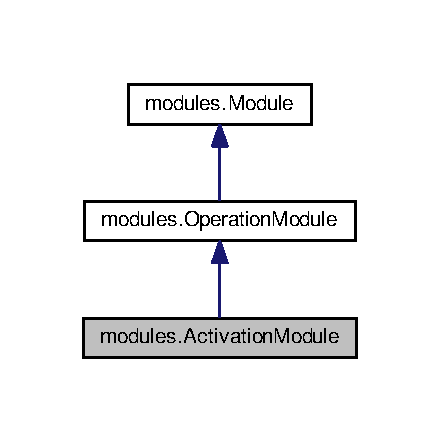
\includegraphics[width=211pt]{classmodules_1_1_activation_module__inherit__graph}
\end{center}
\end{figure}
\subsection*{Public Member Functions}
\begin{DoxyCompactItemize}
\item 
def \hyperlink{classmodules_1_1_activation_module_a8de2b8f05ce37f9d874b4a9872dc0b5e}{\+\_\+\+\_\+init\+\_\+\+\_\+} (self, name, activation)
\item 
\mbox{\Hypertarget{classmodules_1_1_activation_module_a7c4940fe0bde2e70efa8b95a79cfa4d1}\label{classmodules_1_1_activation_module_a7c4940fe0bde2e70efa8b95a79cfa4d1}} 
def \hyperlink{classmodules_1_1_activation_module_a7c4940fe0bde2e70efa8b95a79cfa4d1}{operation} (self, x)
\begin{DoxyCompactList}\small\item\em returns the resulting tensor after applying the activation function \end{DoxyCompactList}\end{DoxyCompactItemize}
\subsection*{Public Attributes}
\begin{DoxyCompactItemize}
\item 
\mbox{\Hypertarget{classmodules_1_1_activation_module_acc7b47491ec7f994594f9e0d2996f61e}\label{classmodules_1_1_activation_module_acc7b47491ec7f994594f9e0d2996f61e}} 
{\bfseries activation}
\end{DoxyCompactItemize}


\subsection{Detailed Description}
Apply an activation function on its input module. 

\subsection{Constructor \& Destructor Documentation}
\mbox{\Hypertarget{classmodules_1_1_activation_module_a8de2b8f05ce37f9d874b4a9872dc0b5e}\label{classmodules_1_1_activation_module_a8de2b8f05ce37f9d874b4a9872dc0b5e}} 
\index{modules\+::\+Activation\+Module@{modules\+::\+Activation\+Module}!\+\_\+\+\_\+init\+\_\+\+\_\+@{\+\_\+\+\_\+init\+\_\+\+\_\+}}
\index{\+\_\+\+\_\+init\+\_\+\+\_\+@{\+\_\+\+\_\+init\+\_\+\+\_\+}!modules\+::\+Activation\+Module@{modules\+::\+Activation\+Module}}
\subsubsection{\texorpdfstring{\+\_\+\+\_\+init\+\_\+\+\_\+()}{\_\_init\_\_()}}
{\footnotesize\ttfamily def modules.\+Activation\+Module.\+\_\+\+\_\+init\+\_\+\+\_\+ (\begin{DoxyParamCaption}\item[{}]{self,  }\item[{}]{name,  }\item[{}]{activation }\end{DoxyParamCaption})}


\begin{DoxyParams}{Parameters}
{\em activation} & callable, a tensorflow function \\
\hline
\end{DoxyParams}


The documentation for this class was generated from the following file\+:\begin{DoxyCompactItemize}
\item 
/home/cwilmot/\+Documents/\+F\+I\+A\+S/phd/code/python/modules/src/modules.\+py\end{DoxyCompactItemize}

\hypertarget{classmodules_1_1_add_module}{}\section{modules.\+Add\+Module Class Reference}
\label{classmodules_1_1_add_module}\index{modules.\+Add\+Module@{modules.\+Add\+Module}}


This module computes the sum of all its input.  




Inheritance diagram for modules.\+Add\+Module\+:\nopagebreak
\begin{figure}[H]
\begin{center}
\leavevmode
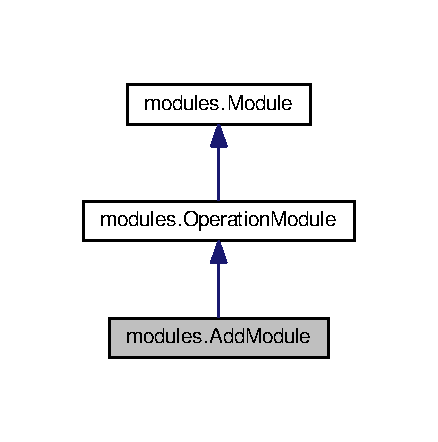
\includegraphics[width=210pt]{classmodules_1_1_add_module__inherit__graph}
\end{center}
\end{figure}
\subsection*{Public Member Functions}
\begin{DoxyCompactItemize}
\item 
\mbox{\Hypertarget{classmodules_1_1_add_module_a3876b3edcfd11f0a993288516ed62449}\label{classmodules_1_1_add_module_a3876b3edcfd11f0a993288516ed62449}} 
def \hyperlink{classmodules_1_1_add_module_a3876b3edcfd11f0a993288516ed62449}{operation} (self, args)
\begin{DoxyCompactList}\small\item\em returns the sum of the output tensors of all its input modules \end{DoxyCompactList}\end{DoxyCompactItemize}
\subsection*{Additional Inherited Members}


\subsection{Detailed Description}
This module computes the sum of all its input. 

It can have as many inputs as requiered and does not support recursions 

The documentation for this class was generated from the following file\+:\begin{DoxyCompactItemize}
\item 
/home/cwilmot/\+Documents/\+F\+I\+A\+S/phd/code/python/modules/src/modules.\+py\end{DoxyCompactItemize}

\hypertarget{classmodules_1_1_batch_accuracy_module}{}\section{modules.\+Batch\+Accuracy\+Module Class Reference}
\label{classmodules_1_1_batch_accuracy_module}\index{modules.\+Batch\+Accuracy\+Module@{modules.\+Batch\+Accuracy\+Module}}


\hyperlink{classmodules_1_1_module}{Module} to compute the classification accuracy.  




Inheritance diagram for modules.\+Batch\+Accuracy\+Module\+:\nopagebreak
\begin{figure}[H]
\begin{center}
\leavevmode
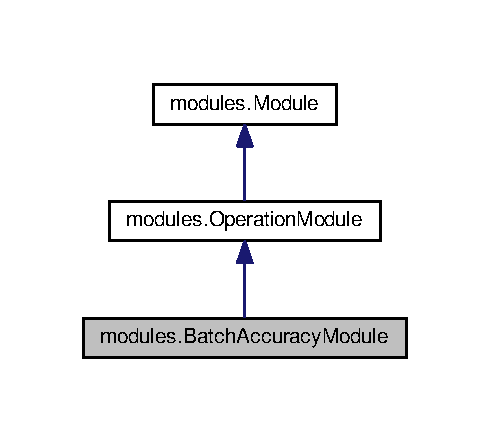
\includegraphics[width=235pt]{classmodules_1_1_batch_accuracy_module__inherit__graph}
\end{center}
\end{figure}
\subsection*{Public Member Functions}
\begin{DoxyCompactItemize}
\item 
\mbox{\Hypertarget{classmodules_1_1_batch_accuracy_module_abb6f5b1c6d8e93ddec73bd8a69453da8}\label{classmodules_1_1_batch_accuracy_module_abb6f5b1c6d8e93ddec73bd8a69453da8}} 
def \hyperlink{classmodules_1_1_batch_accuracy_module_abb6f5b1c6d8e93ddec73bd8a69453da8}{operation} (self, x1, x2)
\begin{DoxyCompactList}\small\item\em returns a tensorflow tensor which holds the accuracy (scalar) \end{DoxyCompactList}\end{DoxyCompactItemize}
\subsection*{Additional Inherited Members}


\subsection{Detailed Description}
\hyperlink{classmodules_1_1_module}{Module} to compute the classification accuracy. 

This modules takes exactly two input modules (two one-\/hot tensors to compare) 

The documentation for this class was generated from the following file\+:\begin{DoxyCompactItemize}
\item 
/home/cwilmot/\+Documents/\+F\+I\+A\+S/phd/code/python/modules/src/modules.\+py\end{DoxyCompactItemize}

\hypertarget{classmodules_1_1_bias_module}{}\section{modules.\+Bias\+Module Class Reference}
\label{classmodules_1_1_bias_module}\index{modules.\+Bias\+Module@{modules.\+Bias\+Module}}


\hyperlink{classmodules_1_1_module}{Module} to create a bias, that can be added to an other tensor inputs modules of this module are not taken into account.  




Inheritance diagram for modules.\+Bias\+Module\+:\nopagebreak
\begin{figure}[H]
\begin{center}
\leavevmode
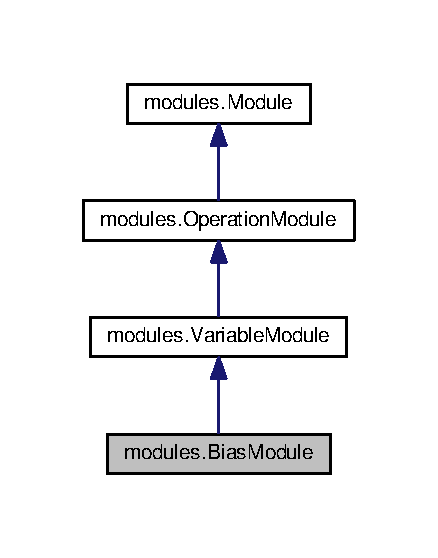
\includegraphics[width=210pt]{classmodules_1_1_bias_module__inherit__graph}
\end{center}
\end{figure}
\subsection*{Public Member Functions}
\begin{DoxyCompactItemize}
\item 
def \hyperlink{classmodules_1_1_bias_module_a680a602fe8d3f45ef483964d1b30e42b}{\+\_\+\+\_\+init\+\_\+\+\_\+} (self, name, bias\+\_\+shape)
\item 
\mbox{\Hypertarget{classmodules_1_1_bias_module_a1cfd19d6bc40759cb6a8127d50c34a80}\label{classmodules_1_1_bias_module_a1cfd19d6bc40759cb6a8127d50c34a80}} 
def \hyperlink{classmodules_1_1_bias_module_a1cfd19d6bc40759cb6a8127d50c34a80}{operation} (self, args)
\begin{DoxyCompactList}\small\item\em Always return the tensorflow Variable which holds the bias. \end{DoxyCompactList}\item 
\mbox{\Hypertarget{classmodules_1_1_bias_module_ae304d936f9ef989264d4be74f41282ac}\label{classmodules_1_1_bias_module_ae304d936f9ef989264d4be74f41282ac}} 
def \hyperlink{classmodules_1_1_bias_module_ae304d936f9ef989264d4be74f41282ac}{create\+\_\+variables} (self, name)
\begin{DoxyCompactList}\small\item\em instanciate the tensorflow Varaible with the shape specified in the constructor \end{DoxyCompactList}\end{DoxyCompactItemize}
\subsection*{Public Attributes}
\begin{DoxyCompactItemize}
\item 
\mbox{\Hypertarget{classmodules_1_1_bias_module_a1ee79711d62e3e8e13bec2e9f3a2cf98}\label{classmodules_1_1_bias_module_a1ee79711d62e3e8e13bec2e9f3a2cf98}} 
{\bfseries bias\+\_\+shape}
\item 
\mbox{\Hypertarget{classmodules_1_1_bias_module_a9b6d3fe09f56ef6ef266c1d6e22f8893}\label{classmodules_1_1_bias_module_a9b6d3fe09f56ef6ef266c1d6e22f8893}} 
{\bfseries bias}
\end{DoxyCompactItemize}


\subsection{Detailed Description}
\hyperlink{classmodules_1_1_module}{Module} to create a bias, that can be added to an other tensor inputs modules of this module are not taken into account. 

\subsection{Constructor \& Destructor Documentation}
\mbox{\Hypertarget{classmodules_1_1_bias_module_a680a602fe8d3f45ef483964d1b30e42b}\label{classmodules_1_1_bias_module_a680a602fe8d3f45ef483964d1b30e42b}} 
\index{modules\+::\+Bias\+Module@{modules\+::\+Bias\+Module}!\+\_\+\+\_\+init\+\_\+\+\_\+@{\+\_\+\+\_\+init\+\_\+\+\_\+}}
\index{\+\_\+\+\_\+init\+\_\+\+\_\+@{\+\_\+\+\_\+init\+\_\+\+\_\+}!modules\+::\+Bias\+Module@{modules\+::\+Bias\+Module}}
\subsubsection{\texorpdfstring{\+\_\+\+\_\+init\+\_\+\+\_\+()}{\_\_init\_\_()}}
{\footnotesize\ttfamily def modules.\+Bias\+Module.\+\_\+\+\_\+init\+\_\+\+\_\+ (\begin{DoxyParamCaption}\item[{}]{self,  }\item[{}]{name,  }\item[{}]{bias\+\_\+shape }\end{DoxyParamCaption})}


\begin{DoxyParams}{Parameters}
{\em bias\+\_\+shape} & tuple, list or np.\+array, the shape of the bias \\
\hline
\end{DoxyParams}


The documentation for this class was generated from the following file\+:\begin{DoxyCompactItemize}
\item 
/home/cwilmot/\+Documents/\+F\+I\+A\+S/phd/code/python/modules/src/modules.\+py\end{DoxyCompactItemize}

\hypertarget{classmodules_1_1_composed_module}{}\section{modules.\+Composed\+Module Class Reference}
\label{classmodules_1_1_composed_module}\index{modules.\+Composed\+Module@{modules.\+Composed\+Module}}


This class is an abstract class which allows when overwritten to create a module that is composed of other modules and does not accept recursions See the implementation of \hyperlink{classmodules_1_1_convolutional_layer_module}{Convolutional\+Layer\+Module} for more info.  




Inheritance diagram for modules.\+Composed\+Module\+:\nopagebreak
\begin{figure}[H]
\begin{center}
\leavevmode
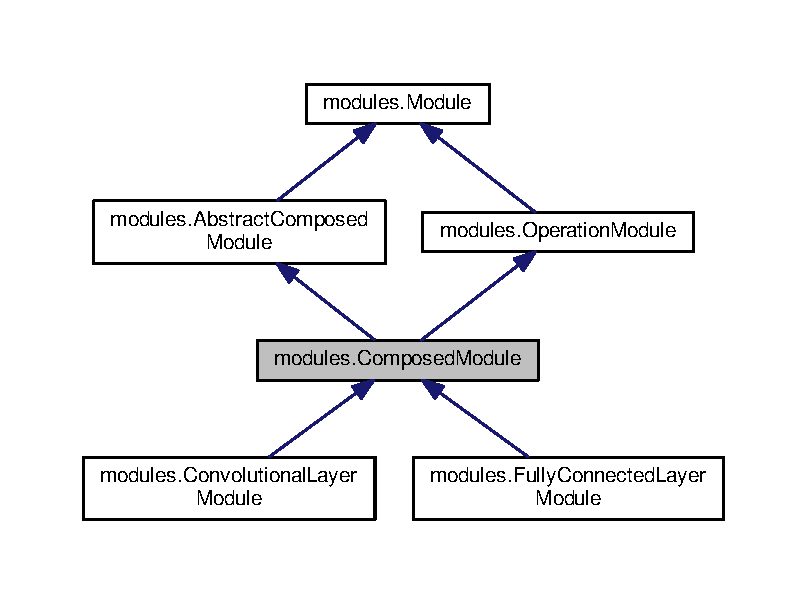
\includegraphics[width=350pt]{classmodules_1_1_composed_module__inherit__graph}
\end{center}
\end{figure}
\subsection*{Additional Inherited Members}


\subsection{Detailed Description}
This class is an abstract class which allows when overwritten to create a module that is composed of other modules and does not accept recursions See the implementation of \hyperlink{classmodules_1_1_convolutional_layer_module}{Convolutional\+Layer\+Module} for more info. 

the methode \textquotesingle{}define\+\_\+inner\+\_\+modules\textquotesingle{} must be overwritten, the attribute input\+\_\+module must be set to the module which is the input of the composed module the attribute output\+\_\+module must be set to the module which is the output of the composed module 

The documentation for this class was generated from the following file\+:\begin{DoxyCompactItemize}
\item 
/home/cwilmot/\+Documents/\+F\+I\+A\+S/phd/code/python/modules/src/modules.\+py\end{DoxyCompactItemize}

\hypertarget{classmodules_1_1_constant_placeholder_module}{}\section{modules.\+Constant\+Placeholder\+Module Class Reference}
\label{classmodules_1_1_constant_placeholder_module}\index{modules.\+Constant\+Placeholder\+Module@{modules.\+Constant\+Placeholder\+Module}}


\hyperlink{classmodules_1_1_module}{Module} to reserve a place to feed in data.  




Inheritance diagram for modules.\+Constant\+Placeholder\+Module\+:\nopagebreak
\begin{figure}[H]
\begin{center}
\leavevmode
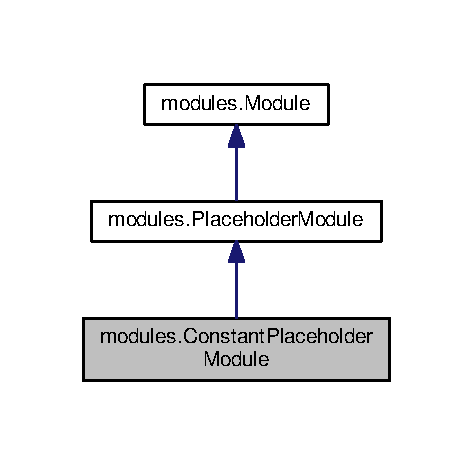
\includegraphics[width=227pt]{classmodules_1_1_constant_placeholder_module__inherit__graph}
\end{center}
\end{figure}
\subsection*{Public Member Functions}
\begin{DoxyCompactItemize}
\item 
\mbox{\Hypertarget{classmodules_1_1_constant_placeholder_module_a901989804cfa2399b0c2888127693589}\label{classmodules_1_1_constant_placeholder_module_a901989804cfa2399b0c2888127693589}} 
def \hyperlink{classmodules_1_1_constant_placeholder_module_a901989804cfa2399b0c2888127693589}{operation} (self)
\begin{DoxyCompactList}\small\item\em always returns the placeholder \end{DoxyCompactList}\end{DoxyCompactItemize}
\subsection*{Additional Inherited Members}


\subsection{Detailed Description}
\hyperlink{classmodules_1_1_module}{Module} to reserve a place to feed in data. 

This module takes no input 

The documentation for this class was generated from the following file\+:\begin{DoxyCompactItemize}
\item 
/home/cwilmot/\+Documents/\+F\+I\+A\+S/phd/code/python/modules/src/modules.\+py\end{DoxyCompactItemize}

\hypertarget{classmodules_1_1_conv2_d_module}{}\section{modules.\+Conv2\+D\+Module Class Reference}
\label{classmodules_1_1_conv2_d_module}\index{modules.\+Conv2\+D\+Module@{modules.\+Conv2\+D\+Module}}


\hyperlink{classmodules_1_1_module}{Module} to perform a convolution.  




Inheritance diagram for modules.\+Conv2\+D\+Module\+:\nopagebreak
\begin{figure}[H]
\begin{center}
\leavevmode
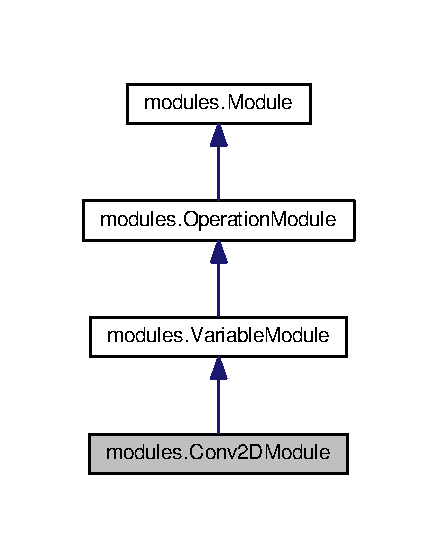
\includegraphics[width=210pt]{classmodules_1_1_conv2_d_module__inherit__graph}
\end{center}
\end{figure}
\subsection*{Public Member Functions}
\begin{DoxyCompactItemize}
\item 
\mbox{\Hypertarget{classmodules_1_1_conv2_d_module_a4b8ae22ca179fb5dd43308be41a6cd69}\label{classmodules_1_1_conv2_d_module_a4b8ae22ca179fb5dd43308be41a6cd69}} 
def \hyperlink{classmodules_1_1_conv2_d_module_a4b8ae22ca179fb5dd43308be41a6cd69}{\+\_\+\+\_\+init\+\_\+\+\_\+} (self, name, filter\+\_\+shape, strides, padding=\textquotesingle{}S\+A\+ME\textquotesingle{})
\begin{DoxyCompactList}\small\item\em It takes the same argument as the tensorflow conv2d. \end{DoxyCompactList}\item 
def \hyperlink{classmodules_1_1_conv2_d_module_a076958c1410647dd4e7982c61c72585f}{operation} (self, x)
\begin{DoxyCompactList}\small\item\em Perform a convolution on the output tensor of the input module in the current time slice. \end{DoxyCompactList}\item 
\mbox{\Hypertarget{classmodules_1_1_conv2_d_module_a03aef9494daf02037d2b2eb581e5eb42}\label{classmodules_1_1_conv2_d_module_a03aef9494daf02037d2b2eb581e5eb42}} 
def \hyperlink{classmodules_1_1_conv2_d_module_a03aef9494daf02037d2b2eb581e5eb42}{create\+\_\+variables} (self, name)
\begin{DoxyCompactList}\small\item\em Creates the filters (or weights) for the convolution according to the parameters given in the constructor. \end{DoxyCompactList}\end{DoxyCompactItemize}
\subsection*{Public Attributes}
\begin{DoxyCompactItemize}
\item 
\mbox{\Hypertarget{classmodules_1_1_conv2_d_module_a90ed6577efa095e41c0469bbe3cdc36b}\label{classmodules_1_1_conv2_d_module_a90ed6577efa095e41c0469bbe3cdc36b}} 
{\bfseries filter\+\_\+shape}
\item 
\mbox{\Hypertarget{classmodules_1_1_conv2_d_module_a0f17e4adfc620cb0dbf4e66edf8b2411}\label{classmodules_1_1_conv2_d_module_a0f17e4adfc620cb0dbf4e66edf8b2411}} 
{\bfseries strides}
\item 
\mbox{\Hypertarget{classmodules_1_1_conv2_d_module_a937db3136e264bf649567930729a3491}\label{classmodules_1_1_conv2_d_module_a937db3136e264bf649567930729a3491}} 
{\bfseries padding}
\item 
\mbox{\Hypertarget{classmodules_1_1_conv2_d_module_a6efceb0b6be04ded563de096808f7e0e}\label{classmodules_1_1_conv2_d_module_a6efceb0b6be04ded563de096808f7e0e}} 
{\bfseries weights}
\end{DoxyCompactItemize}


\subsection{Detailed Description}
\hyperlink{classmodules_1_1_module}{Module} to perform a convolution. 

This module can have a single input module 

\subsection{Member Function Documentation}
\mbox{\Hypertarget{classmodules_1_1_conv2_d_module_a076958c1410647dd4e7982c61c72585f}\label{classmodules_1_1_conv2_d_module_a076958c1410647dd4e7982c61c72585f}} 
\index{modules\+::\+Conv2\+D\+Module@{modules\+::\+Conv2\+D\+Module}!operation@{operation}}
\index{operation@{operation}!modules\+::\+Conv2\+D\+Module@{modules\+::\+Conv2\+D\+Module}}
\subsubsection{\texorpdfstring{operation()}{operation()}}
{\footnotesize\ttfamily def modules.\+Conv2\+D\+Module.\+operation (\begin{DoxyParamCaption}\item[{}]{self,  }\item[{}]{x }\end{DoxyParamCaption})}



Perform a convolution on the output tensor of the input module in the current time slice. 

This module can have a single input module. 

The documentation for this class was generated from the following file\+:\begin{DoxyCompactItemize}
\item 
/home/cwilmot/\+Documents/\+F\+I\+A\+S/phd/code/python/modules/src/modules.\+py\end{DoxyCompactItemize}

\hypertarget{classmodules_1_1_conv2_d_transpose_module}{}\section{modules.\+Conv2\+D\+Transpose\+Module Class Reference}
\label{classmodules_1_1_conv2_d_transpose_module}\index{modules.\+Conv2\+D\+Transpose\+Module@{modules.\+Conv2\+D\+Transpose\+Module}}


\hyperlink{classmodules_1_1_module}{Module} to perform a deconvolution.  




Inheritance diagram for modules.\+Conv2\+D\+Transpose\+Module\+:\nopagebreak
\begin{figure}[H]
\begin{center}
\leavevmode
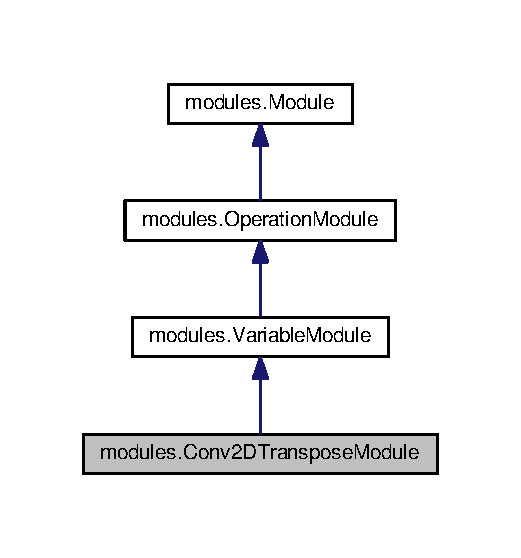
\includegraphics[width=250pt]{classmodules_1_1_conv2_d_transpose_module__inherit__graph}
\end{center}
\end{figure}
\subsection*{Public Member Functions}
\begin{DoxyCompactItemize}
\item 
\mbox{\Hypertarget{classmodules_1_1_conv2_d_transpose_module_acdba05e0c793a743336082c4778ef125}\label{classmodules_1_1_conv2_d_transpose_module_acdba05e0c793a743336082c4778ef125}} 
def \hyperlink{classmodules_1_1_conv2_d_transpose_module_acdba05e0c793a743336082c4778ef125}{\+\_\+\+\_\+init\+\_\+\+\_\+} (self, name, filter\+\_\+shape, strides, output\+\_\+shape, padding=\textquotesingle{}S\+A\+ME\textquotesingle{})
\begin{DoxyCompactList}\small\item\em It takes the same argument as the tensorflow conv2d\+\_\+transpose. \end{DoxyCompactList}\item 
def \hyperlink{classmodules_1_1_conv2_d_transpose_module_a39b975d02ff419a91c3e5e9addd5aa18}{operation} (self, x)
\begin{DoxyCompactList}\small\item\em Perform a deconvolution on the output tensor of the input module in the current time slice. \end{DoxyCompactList}\item 
\mbox{\Hypertarget{classmodules_1_1_conv2_d_transpose_module_af4d9c9bcb7a6e234a40d8027e64456e8}\label{classmodules_1_1_conv2_d_transpose_module_af4d9c9bcb7a6e234a40d8027e64456e8}} 
def \hyperlink{classmodules_1_1_conv2_d_transpose_module_af4d9c9bcb7a6e234a40d8027e64456e8}{create\+\_\+variables} (self, name)
\begin{DoxyCompactList}\small\item\em Creates the filters (or weights) for the deconvolution according to the parameters given in the constructor. \end{DoxyCompactList}\end{DoxyCompactItemize}
\subsection*{Public Attributes}
\begin{DoxyCompactItemize}
\item 
\mbox{\Hypertarget{classmodules_1_1_conv2_d_transpose_module_adc3ca12449e5a7ef8456f0e2332075a6}\label{classmodules_1_1_conv2_d_transpose_module_adc3ca12449e5a7ef8456f0e2332075a6}} 
{\bfseries filter\+\_\+shape}
\item 
\mbox{\Hypertarget{classmodules_1_1_conv2_d_transpose_module_a885a832074360edfb622eb40b4cbc8ee}\label{classmodules_1_1_conv2_d_transpose_module_a885a832074360edfb622eb40b4cbc8ee}} 
{\bfseries strides}
\item 
\mbox{\Hypertarget{classmodules_1_1_conv2_d_transpose_module_a8dfce8281b7bd58a9797b84c1f3f94cc}\label{classmodules_1_1_conv2_d_transpose_module_a8dfce8281b7bd58a9797b84c1f3f94cc}} 
{\bfseries output\+\_\+shape}
\item 
\mbox{\Hypertarget{classmodules_1_1_conv2_d_transpose_module_ab207775ad3259edda6cb6fc01b5e67f0}\label{classmodules_1_1_conv2_d_transpose_module_ab207775ad3259edda6cb6fc01b5e67f0}} 
{\bfseries padding}
\item 
\mbox{\Hypertarget{classmodules_1_1_conv2_d_transpose_module_a160963233d3a6e83ab47917a28b7bcac}\label{classmodules_1_1_conv2_d_transpose_module_a160963233d3a6e83ab47917a28b7bcac}} 
{\bfseries weights}
\end{DoxyCompactItemize}


\subsection{Detailed Description}
\hyperlink{classmodules_1_1_module}{Module} to perform a deconvolution. 

This module can have a single input module 

\subsection{Member Function Documentation}
\mbox{\Hypertarget{classmodules_1_1_conv2_d_transpose_module_a39b975d02ff419a91c3e5e9addd5aa18}\label{classmodules_1_1_conv2_d_transpose_module_a39b975d02ff419a91c3e5e9addd5aa18}} 
\index{modules\+::\+Conv2\+D\+Transpose\+Module@{modules\+::\+Conv2\+D\+Transpose\+Module}!operation@{operation}}
\index{operation@{operation}!modules\+::\+Conv2\+D\+Transpose\+Module@{modules\+::\+Conv2\+D\+Transpose\+Module}}
\subsubsection{\texorpdfstring{operation()}{operation()}}
{\footnotesize\ttfamily def modules.\+Conv2\+D\+Transpose\+Module.\+operation (\begin{DoxyParamCaption}\item[{}]{self,  }\item[{}]{x }\end{DoxyParamCaption})}



Perform a deconvolution on the output tensor of the input module in the current time slice. 

This module can have a single input module. 

The documentation for this class was generated from the following file\+:\begin{DoxyCompactItemize}
\item 
/home/cwilmot/\+Documents/\+F\+I\+A\+S/phd/code/python/modules/src/modules.\+py\end{DoxyCompactItemize}

\hypertarget{classmodules_1_1_convolutional_layer_module}{}\section{modules.\+Convolutional\+Layer\+Module Class Reference}
\label{classmodules_1_1_convolutional_layer_module}\index{modules.\+Convolutional\+Layer\+Module@{modules.\+Convolutional\+Layer\+Module}}


This composed module performs a convolution and applies a bias and an activation function.  




Inheritance diagram for modules.\+Convolutional\+Layer\+Module\+:\nopagebreak
\begin{figure}[H]
\begin{center}
\leavevmode
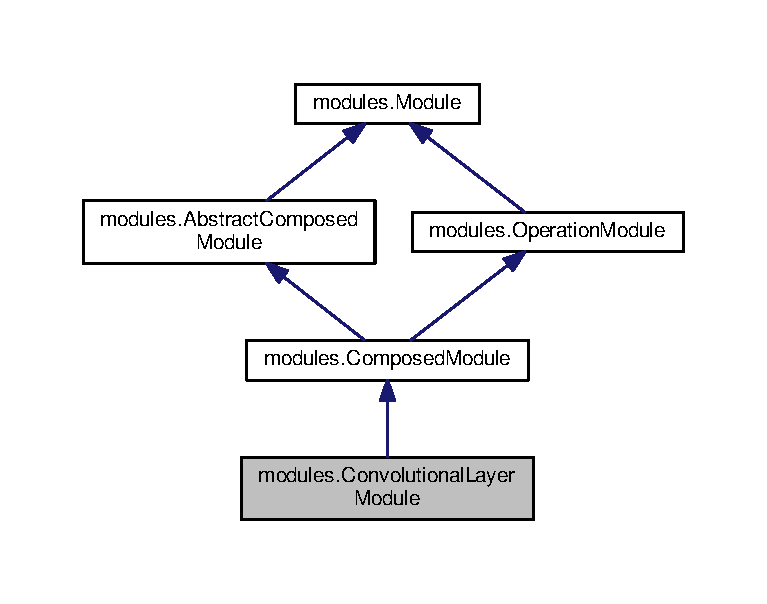
\includegraphics[width=350pt]{classmodules_1_1_convolutional_layer_module__inherit__graph}
\end{center}
\end{figure}
\subsection*{Public Member Functions}
\begin{DoxyCompactItemize}
\item 
\mbox{\Hypertarget{classmodules_1_1_convolutional_layer_module_aaa6eabaf3b9d4058bc29e11a49132170}\label{classmodules_1_1_convolutional_layer_module_aaa6eabaf3b9d4058bc29e11a49132170}} 
def {\bfseries define\+\_\+inner\+\_\+modules} (self, name, activation, filter\+\_\+shape, strides, bias\+\_\+shape, padding=\textquotesingle{}S\+A\+ME\textquotesingle{})
\end{DoxyCompactItemize}
\subsection*{Public Attributes}
\begin{DoxyCompactItemize}
\item 
\mbox{\Hypertarget{classmodules_1_1_convolutional_layer_module_aa63060498756e70cf6b9c735c35d9dbd}\label{classmodules_1_1_convolutional_layer_module_aa63060498756e70cf6b9c735c35d9dbd}} 
{\bfseries input\+\_\+module}
\item 
\mbox{\Hypertarget{classmodules_1_1_convolutional_layer_module_ad26604b43fb51440c378aac5b8d0cfe4}\label{classmodules_1_1_convolutional_layer_module_ad26604b43fb51440c378aac5b8d0cfe4}} 
{\bfseries bias}
\item 
\mbox{\Hypertarget{classmodules_1_1_convolutional_layer_module_a2d61b622c129b7608c76070de958560e}\label{classmodules_1_1_convolutional_layer_module_a2d61b622c129b7608c76070de958560e}} 
{\bfseries preactivation}
\item 
\mbox{\Hypertarget{classmodules_1_1_convolutional_layer_module_a12317713722fd8c7e760c509ea83c214}\label{classmodules_1_1_convolutional_layer_module_a12317713722fd8c7e760c509ea83c214}} 
{\bfseries output\+\_\+module}
\end{DoxyCompactItemize}


\subsection{Detailed Description}
This composed module performs a convolution and applies a bias and an activation function. 

It does not allow recursions 

The documentation for this class was generated from the following file\+:\begin{DoxyCompactItemize}
\item 
/home/cwilmot/\+Documents/\+F\+I\+A\+S/phd/code/python/modules/src/modules.\+py\end{DoxyCompactItemize}

\hypertarget{classmodules_1_1_error_module}{}\section{modules.\+Error\+Module Class Reference}
\label{classmodules_1_1_error_module}\index{modules.\+Error\+Module@{modules.\+Error\+Module}}


\hyperlink{classmodules_1_1_module}{Module} to compute an error (or apply any tensorflow operation on two and only two tensors)  




Inheritance diagram for modules.\+Error\+Module\+:\nopagebreak
\begin{figure}[H]
\begin{center}
\leavevmode
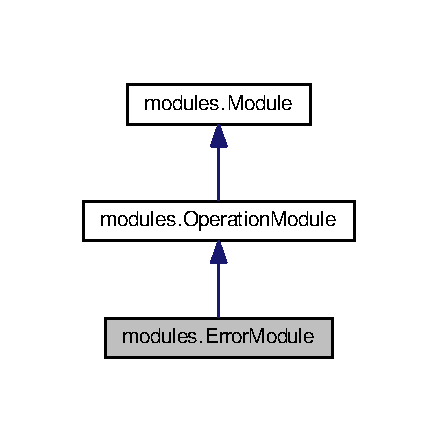
\includegraphics[width=210pt]{classmodules_1_1_error_module__inherit__graph}
\end{center}
\end{figure}
\subsection*{Public Member Functions}
\begin{DoxyCompactItemize}
\item 
def \hyperlink{classmodules_1_1_error_module_ac657fdedba3e5af8e96faf1e9fdfdbdf}{\+\_\+\+\_\+init\+\_\+\+\_\+} (self, name, error\+\_\+func)
\item 
\mbox{\Hypertarget{classmodules_1_1_error_module_a276b0c608f97bafccb52e264f1e2cdfd}\label{classmodules_1_1_error_module_a276b0c608f97bafccb52e264f1e2cdfd}} 
def \hyperlink{classmodules_1_1_error_module_a276b0c608f97bafccb52e264f1e2cdfd}{operation} (self, x1, x2)
\begin{DoxyCompactList}\small\item\em apply the function passed in the constructor its two input modules \end{DoxyCompactList}\end{DoxyCompactItemize}
\subsection*{Public Attributes}
\begin{DoxyCompactItemize}
\item 
\mbox{\Hypertarget{classmodules_1_1_error_module_ac571881352c250096e78a90e1d8c1295}\label{classmodules_1_1_error_module_ac571881352c250096e78a90e1d8c1295}} 
{\bfseries error\+\_\+func}
\end{DoxyCompactItemize}


\subsection{Detailed Description}
\hyperlink{classmodules_1_1_module}{Module} to compute an error (or apply any tensorflow operation on two and only two tensors) 

\subsection{Constructor \& Destructor Documentation}
\mbox{\Hypertarget{classmodules_1_1_error_module_ac657fdedba3e5af8e96faf1e9fdfdbdf}\label{classmodules_1_1_error_module_ac657fdedba3e5af8e96faf1e9fdfdbdf}} 
\index{modules\+::\+Error\+Module@{modules\+::\+Error\+Module}!\+\_\+\+\_\+init\+\_\+\+\_\+@{\+\_\+\+\_\+init\+\_\+\+\_\+}}
\index{\+\_\+\+\_\+init\+\_\+\+\_\+@{\+\_\+\+\_\+init\+\_\+\+\_\+}!modules\+::\+Error\+Module@{modules\+::\+Error\+Module}}
\subsubsection{\texorpdfstring{\+\_\+\+\_\+init\+\_\+\+\_\+()}{\_\_init\_\_()}}
{\footnotesize\ttfamily def modules.\+Error\+Module.\+\_\+\+\_\+init\+\_\+\+\_\+ (\begin{DoxyParamCaption}\item[{}]{self,  }\item[{}]{name,  }\item[{}]{error\+\_\+func }\end{DoxyParamCaption})}


\begin{DoxyParams}{Parameters}
{\em error\+\_\+func} & callable, function that takes exactly 2 arguments and returns a tensorflow tensor. \\
\hline
\end{DoxyParams}


The documentation for this class was generated from the following file\+:\begin{DoxyCompactItemize}
\item 
/home/cwilmot/\+Documents/\+F\+I\+A\+S/phd/code/python/modules/src/modules.\+py\end{DoxyCompactItemize}

\hypertarget{classmodules_1_1_fake_module}{}\section{modules.\+Fake\+Module Class Reference}
\label{classmodules_1_1_fake_module}\index{modules.\+Fake\+Module@{modules.\+Fake\+Module}}


For testing purpose only, does nothing.  




Inheritance diagram for modules.\+Fake\+Module\+:\nopagebreak
\begin{figure}[H]
\begin{center}
\leavevmode
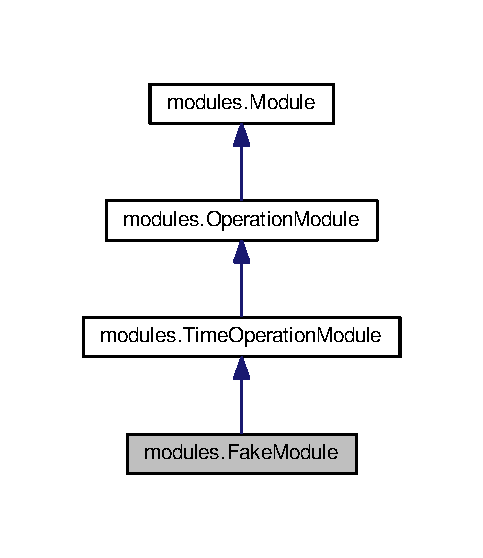
\includegraphics[width=232pt]{classmodules_1_1_fake_module__inherit__graph}
\end{center}
\end{figure}
\subsection*{Public Member Functions}
\begin{DoxyCompactItemize}
\item 
\mbox{\Hypertarget{classmodules_1_1_fake_module_a3a458b0dd01068a669f85be3b0a85aa1}\label{classmodules_1_1_fake_module_a3a458b0dd01068a669f85be3b0a85aa1}} 
def {\bfseries operation} (self, args)
\end{DoxyCompactItemize}
\subsection*{Additional Inherited Members}


\subsection{Detailed Description}
For testing purpose only, does nothing. 

The documentation for this class was generated from the following file\+:\begin{DoxyCompactItemize}
\item 
/home/cwilmot/\+Documents/\+F\+I\+A\+S/phd/code/python/modules/src/modules.\+py\end{DoxyCompactItemize}

\hypertarget{classmodules_1_1_flatten_module}{}\section{modules.\+Flatten\+Module Class Reference}
\label{classmodules_1_1_flatten_module}\index{modules.\+Flatten\+Module@{modules.\+Flatten\+Module}}


\hyperlink{classmodules_1_1_module}{Module} to flatten the output of the input module.  




Inheritance diagram for modules.\+Flatten\+Module\+:\nopagebreak
\begin{figure}[H]
\begin{center}
\leavevmode
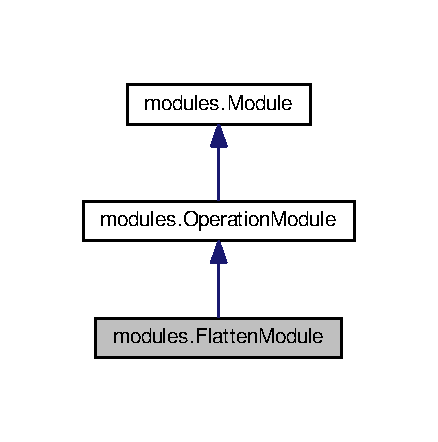
\includegraphics[width=210pt]{classmodules_1_1_flatten_module__inherit__graph}
\end{center}
\end{figure}
\subsection*{Public Member Functions}
\begin{DoxyCompactItemize}
\item 
\mbox{\Hypertarget{classmodules_1_1_flatten_module_a591c52c7ecfcd1f52730d5eb453199d2}\label{classmodules_1_1_flatten_module_a591c52c7ecfcd1f52730d5eb453199d2}} 
def \hyperlink{classmodules_1_1_flatten_module_a591c52c7ecfcd1f52730d5eb453199d2}{operation} (self, x)
\begin{DoxyCompactList}\small\item\em Returns the reshaped output tensor of the input module. \end{DoxyCompactList}\end{DoxyCompactItemize}
\subsection*{Additional Inherited Members}


\subsection{Detailed Description}
\hyperlink{classmodules_1_1_module}{Module} to flatten the output of the input module. 

It useful for example to perform a fully connected layer after a convolutional layer 

The documentation for this class was generated from the following file\+:\begin{DoxyCompactItemize}
\item 
/home/cwilmot/\+Documents/\+F\+I\+A\+S/phd/code/python/modules/src/modules.\+py\end{DoxyCompactItemize}

\hypertarget{classmodules_1_1_fully_connected_layer_module}{}\section{modules.\+Fully\+Connected\+Layer\+Module Class Reference}
\label{classmodules_1_1_fully_connected_layer_module}\index{modules.\+Fully\+Connected\+Layer\+Module@{modules.\+Fully\+Connected\+Layer\+Module}}


This composed module performs a full connection and applies a bias and an activation function.  




Inheritance diagram for modules.\+Fully\+Connected\+Layer\+Module\+:\nopagebreak
\begin{figure}[H]
\begin{center}
\leavevmode
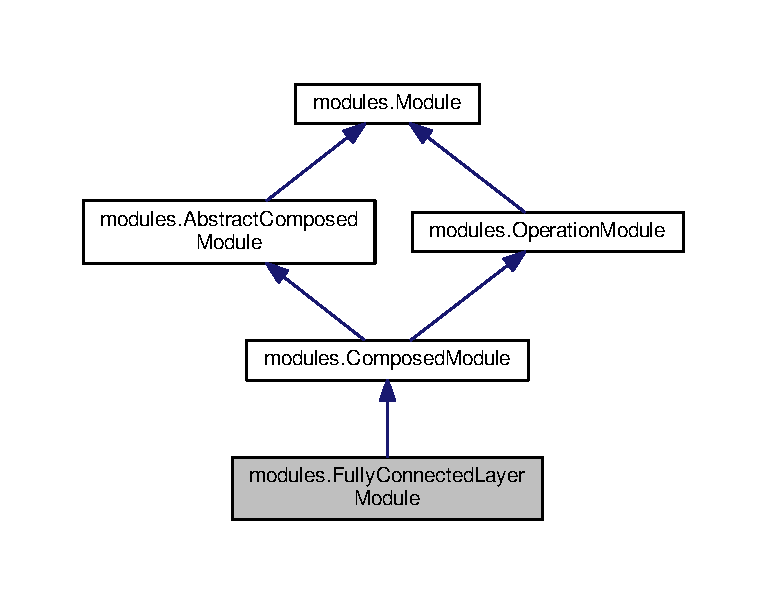
\includegraphics[width=350pt]{classmodules_1_1_fully_connected_layer_module__inherit__graph}
\end{center}
\end{figure}
\subsection*{Public Member Functions}
\begin{DoxyCompactItemize}
\item 
\mbox{\Hypertarget{classmodules_1_1_fully_connected_layer_module_ab2470e07b8f4dd9d8fd924c1f1df0cc3}\label{classmodules_1_1_fully_connected_layer_module_ab2470e07b8f4dd9d8fd924c1f1df0cc3}} 
def {\bfseries define\+\_\+inner\+\_\+modules} (self, name, activation, in\+\_\+size, out\+\_\+size)
\end{DoxyCompactItemize}
\subsection*{Public Attributes}
\begin{DoxyCompactItemize}
\item 
\mbox{\Hypertarget{classmodules_1_1_fully_connected_layer_module_a2fbb4bd59e3e033aa548fdcb7841a19a}\label{classmodules_1_1_fully_connected_layer_module_a2fbb4bd59e3e033aa548fdcb7841a19a}} 
{\bfseries input\+\_\+module}
\item 
\mbox{\Hypertarget{classmodules_1_1_fully_connected_layer_module_ac07d3608d761a0e7da5549323fbc54b5}\label{classmodules_1_1_fully_connected_layer_module_ac07d3608d761a0e7da5549323fbc54b5}} 
{\bfseries bias}
\item 
\mbox{\Hypertarget{classmodules_1_1_fully_connected_layer_module_aa8edd562a443167aefb9be97539617c9}\label{classmodules_1_1_fully_connected_layer_module_aa8edd562a443167aefb9be97539617c9}} 
{\bfseries preactivation}
\item 
\mbox{\Hypertarget{classmodules_1_1_fully_connected_layer_module_ae69442247979be24dc1c8c3477ae821f}\label{classmodules_1_1_fully_connected_layer_module_ae69442247979be24dc1c8c3477ae821f}} 
{\bfseries output\+\_\+module}
\end{DoxyCompactItemize}


\subsection{Detailed Description}
This composed module performs a full connection and applies a bias and an activation function. 

It does not allow recursions 

The documentation for this class was generated from the following file\+:\begin{DoxyCompactItemize}
\item 
/home/cwilmot/\+Documents/\+F\+I\+A\+S/phd/code/python/modules/src/modules.\+py\end{DoxyCompactItemize}

\hypertarget{classmodules_1_1_fully_connected_module}{}\section{modules.\+Fully\+Connected\+Module Class Reference}
\label{classmodules_1_1_fully_connected_module}\index{modules.\+Fully\+Connected\+Module@{modules.\+Fully\+Connected\+Module}}


\hyperlink{classmodules_1_1_module}{Module} to perform a matrix multiplication.  




Inheritance diagram for modules.\+Fully\+Connected\+Module\+:\nopagebreak
\begin{figure}[H]
\begin{center}
\leavevmode
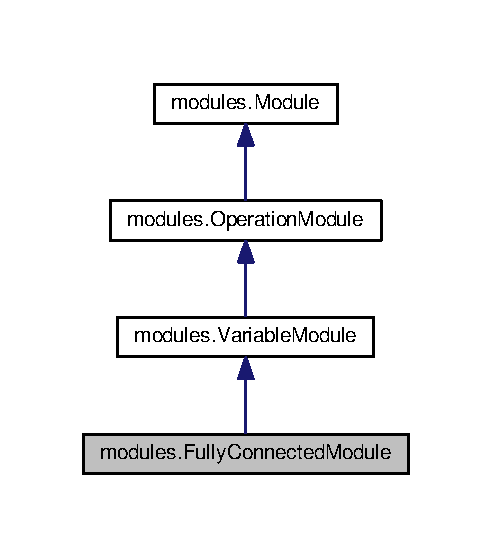
\includegraphics[width=236pt]{classmodules_1_1_fully_connected_module__inherit__graph}
\end{center}
\end{figure}
\subsection*{Public Member Functions}
\begin{DoxyCompactItemize}
\item 
def \hyperlink{classmodules_1_1_fully_connected_module_afb394d5c031fef0fec0feeec80a54fae}{\+\_\+\+\_\+init\+\_\+\+\_\+} (self, name, in\+\_\+size, out\+\_\+size)
\item 
def \hyperlink{classmodules_1_1_fully_connected_module_adb0bf41ff737487804b75ee8bdd9a3b4}{operation} (self, x)
\begin{DoxyCompactList}\small\item\em Returns the matrix multiplication of the output of the input module by a weight matrix. \end{DoxyCompactList}\item 
\mbox{\Hypertarget{classmodules_1_1_fully_connected_module_aafa7090b4a568168526c1782a1b9794f}\label{classmodules_1_1_fully_connected_module_aafa7090b4a568168526c1782a1b9794f}} 
def \hyperlink{classmodules_1_1_fully_connected_module_aafa7090b4a568168526c1782a1b9794f}{create\+\_\+variables} (self, name)
\begin{DoxyCompactList}\small\item\em Instanciate a weight matrix accordingly to the sizes specified in the constructor. \end{DoxyCompactList}\end{DoxyCompactItemize}
\subsection*{Public Attributes}
\begin{DoxyCompactItemize}
\item 
\mbox{\Hypertarget{classmodules_1_1_fully_connected_module_afae1920d4f8094b2bf20677b0e482d2b}\label{classmodules_1_1_fully_connected_module_afae1920d4f8094b2bf20677b0e482d2b}} 
{\bfseries in\+\_\+size}
\item 
\mbox{\Hypertarget{classmodules_1_1_fully_connected_module_abb15a67f0af437ffd177dc2f1c991632}\label{classmodules_1_1_fully_connected_module_abb15a67f0af437ffd177dc2f1c991632}} 
{\bfseries out\+\_\+size}
\item 
\mbox{\Hypertarget{classmodules_1_1_fully_connected_module_ac622fa3065dc7fa896020fd950799480}\label{classmodules_1_1_fully_connected_module_ac622fa3065dc7fa896020fd950799480}} 
{\bfseries weights}
\end{DoxyCompactItemize}


\subsection{Detailed Description}
\hyperlink{classmodules_1_1_module}{Module} to perform a matrix multiplication. 

Again, this module takes a single module as input. 

\subsection{Constructor \& Destructor Documentation}
\mbox{\Hypertarget{classmodules_1_1_fully_connected_module_afb394d5c031fef0fec0feeec80a54fae}\label{classmodules_1_1_fully_connected_module_afb394d5c031fef0fec0feeec80a54fae}} 
\index{modules\+::\+Fully\+Connected\+Module@{modules\+::\+Fully\+Connected\+Module}!\+\_\+\+\_\+init\+\_\+\+\_\+@{\+\_\+\+\_\+init\+\_\+\+\_\+}}
\index{\+\_\+\+\_\+init\+\_\+\+\_\+@{\+\_\+\+\_\+init\+\_\+\+\_\+}!modules\+::\+Fully\+Connected\+Module@{modules\+::\+Fully\+Connected\+Module}}
\subsubsection{\texorpdfstring{\+\_\+\+\_\+init\+\_\+\+\_\+()}{\_\_init\_\_()}}
{\footnotesize\ttfamily def modules.\+Fully\+Connected\+Module.\+\_\+\+\_\+init\+\_\+\+\_\+ (\begin{DoxyParamCaption}\item[{}]{self,  }\item[{}]{name,  }\item[{}]{in\+\_\+size,  }\item[{}]{out\+\_\+size }\end{DoxyParamCaption})}


\begin{DoxyParams}{Parameters}
{\em in\+\_\+size} & int, the number of neurones in the previous layer \\
\hline
{\em out\+\_\+size} & int, the number of neurones in the current new layer \\
\hline
\end{DoxyParams}


\subsection{Member Function Documentation}
\mbox{\Hypertarget{classmodules_1_1_fully_connected_module_adb0bf41ff737487804b75ee8bdd9a3b4}\label{classmodules_1_1_fully_connected_module_adb0bf41ff737487804b75ee8bdd9a3b4}} 
\index{modules\+::\+Fully\+Connected\+Module@{modules\+::\+Fully\+Connected\+Module}!operation@{operation}}
\index{operation@{operation}!modules\+::\+Fully\+Connected\+Module@{modules\+::\+Fully\+Connected\+Module}}
\subsubsection{\texorpdfstring{operation()}{operation()}}
{\footnotesize\ttfamily def modules.\+Fully\+Connected\+Module.\+operation (\begin{DoxyParamCaption}\item[{}]{self,  }\item[{}]{x }\end{DoxyParamCaption})}



Returns the matrix multiplication of the output of the input module by a weight matrix. 



The documentation for this class was generated from the following file\+:\begin{DoxyCompactItemize}
\item 
/home/cwilmot/\+Documents/\+F\+I\+A\+S/phd/code/python/modules/src/modules.\+py\end{DoxyCompactItemize}

\hypertarget{classmodules_1_1_input_container}{}\section{modules.\+Input\+Container Class Reference}
\label{classmodules_1_1_input_container}\index{modules.\+Input\+Container@{modules.\+Input\+Container}}


Inheritance diagram for modules.\+Input\+Container\+:\nopagebreak
\begin{figure}[H]
\begin{center}
\leavevmode
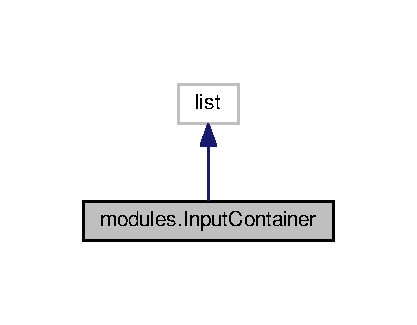
\includegraphics[width=200pt]{classmodules_1_1_input_container__inherit__graph}
\end{center}
\end{figure}
\subsection*{Public Member Functions}
\begin{DoxyCompactItemize}
\item 
\mbox{\Hypertarget{classmodules_1_1_input_container_af7bdc54b020a636c26ca754b7ae15533}\label{classmodules_1_1_input_container_af7bdc54b020a636c26ca754b7ae15533}} 
def {\bfseries \+\_\+\+\_\+iadd\+\_\+\+\_\+} (self, other)
\end{DoxyCompactItemize}


The documentation for this class was generated from the following file\+:\begin{DoxyCompactItemize}
\item 
/home/cwilmot/\+Documents/\+F\+I\+A\+S/phd/code/python/modules/src/modules.\+py\end{DoxyCompactItemize}

\hypertarget{classmodules_1_1_max_pooling_module}{}\section{modules.\+Max\+Pooling\+Module Class Reference}
\label{classmodules_1_1_max_pooling_module}\index{modules.\+Max\+Pooling\+Module@{modules.\+Max\+Pooling\+Module}}


\hyperlink{classmodules_1_1_module}{Module} to perform a maxpooling.  




Inheritance diagram for modules.\+Max\+Pooling\+Module\+:\nopagebreak
\begin{figure}[H]
\begin{center}
\leavevmode
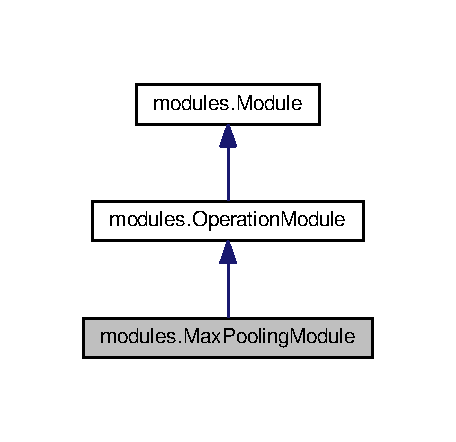
\includegraphics[width=219pt]{classmodules_1_1_max_pooling_module__inherit__graph}
\end{center}
\end{figure}
\subsection*{Public Member Functions}
\begin{DoxyCompactItemize}
\item 
\mbox{\Hypertarget{classmodules_1_1_max_pooling_module_a9542dccd5adecfae6a79f6273e506aa3}\label{classmodules_1_1_max_pooling_module_a9542dccd5adecfae6a79f6273e506aa3}} 
def {\bfseries \+\_\+\+\_\+init\+\_\+\+\_\+} (self, name, ksize, strides, padding=\textquotesingle{}S\+A\+ME\textquotesingle{})
\item 
def \hyperlink{classmodules_1_1_max_pooling_module_a833701a5c7f28279a21984069d3faa11}{operation} (self, x)
\begin{DoxyCompactList}\small\item\em Perform a maxpooling on the output tensor of the input module in the current time slice. \end{DoxyCompactList}\end{DoxyCompactItemize}
\subsection*{Public Attributes}
\begin{DoxyCompactItemize}
\item 
\mbox{\Hypertarget{classmodules_1_1_max_pooling_module_ae007bccfd76c9083d1021643c4969fd4}\label{classmodules_1_1_max_pooling_module_ae007bccfd76c9083d1021643c4969fd4}} 
{\bfseries ksize}
\item 
\mbox{\Hypertarget{classmodules_1_1_max_pooling_module_a234b76388be765dbd5604463e160aca6}\label{classmodules_1_1_max_pooling_module_a234b76388be765dbd5604463e160aca6}} 
{\bfseries strides}
\item 
\mbox{\Hypertarget{classmodules_1_1_max_pooling_module_a719909f20180c9e63249afbe83c409a7}\label{classmodules_1_1_max_pooling_module_a719909f20180c9e63249afbe83c409a7}} 
{\bfseries padding}
\end{DoxyCompactItemize}


\subsection{Detailed Description}
\hyperlink{classmodules_1_1_module}{Module} to perform a maxpooling. 

This module can have a single input module 

\subsection{Member Function Documentation}
\mbox{\Hypertarget{classmodules_1_1_max_pooling_module_a833701a5c7f28279a21984069d3faa11}\label{classmodules_1_1_max_pooling_module_a833701a5c7f28279a21984069d3faa11}} 
\index{modules\+::\+Max\+Pooling\+Module@{modules\+::\+Max\+Pooling\+Module}!operation@{operation}}
\index{operation@{operation}!modules\+::\+Max\+Pooling\+Module@{modules\+::\+Max\+Pooling\+Module}}
\subsubsection{\texorpdfstring{operation()}{operation()}}
{\footnotesize\ttfamily def modules.\+Max\+Pooling\+Module.\+operation (\begin{DoxyParamCaption}\item[{}]{self,  }\item[{}]{x }\end{DoxyParamCaption})}



Perform a maxpooling on the output tensor of the input module in the current time slice. 

This module can have a single input module. 

The documentation for this class was generated from the following file\+:\begin{DoxyCompactItemize}
\item 
/home/cwilmot/\+Documents/\+F\+I\+A\+S/phd/code/python/modules/src/modules.\+py\end{DoxyCompactItemize}

\hypertarget{classmodules_1_1_module}{}\section{modules.\+Module Class Reference}
\label{classmodules_1_1_module}\index{modules.\+Module@{modules.\+Module}}


Base class of a module.  




Inheritance diagram for modules.\+Module\+:\nopagebreak
\begin{figure}[H]
\begin{center}
\leavevmode
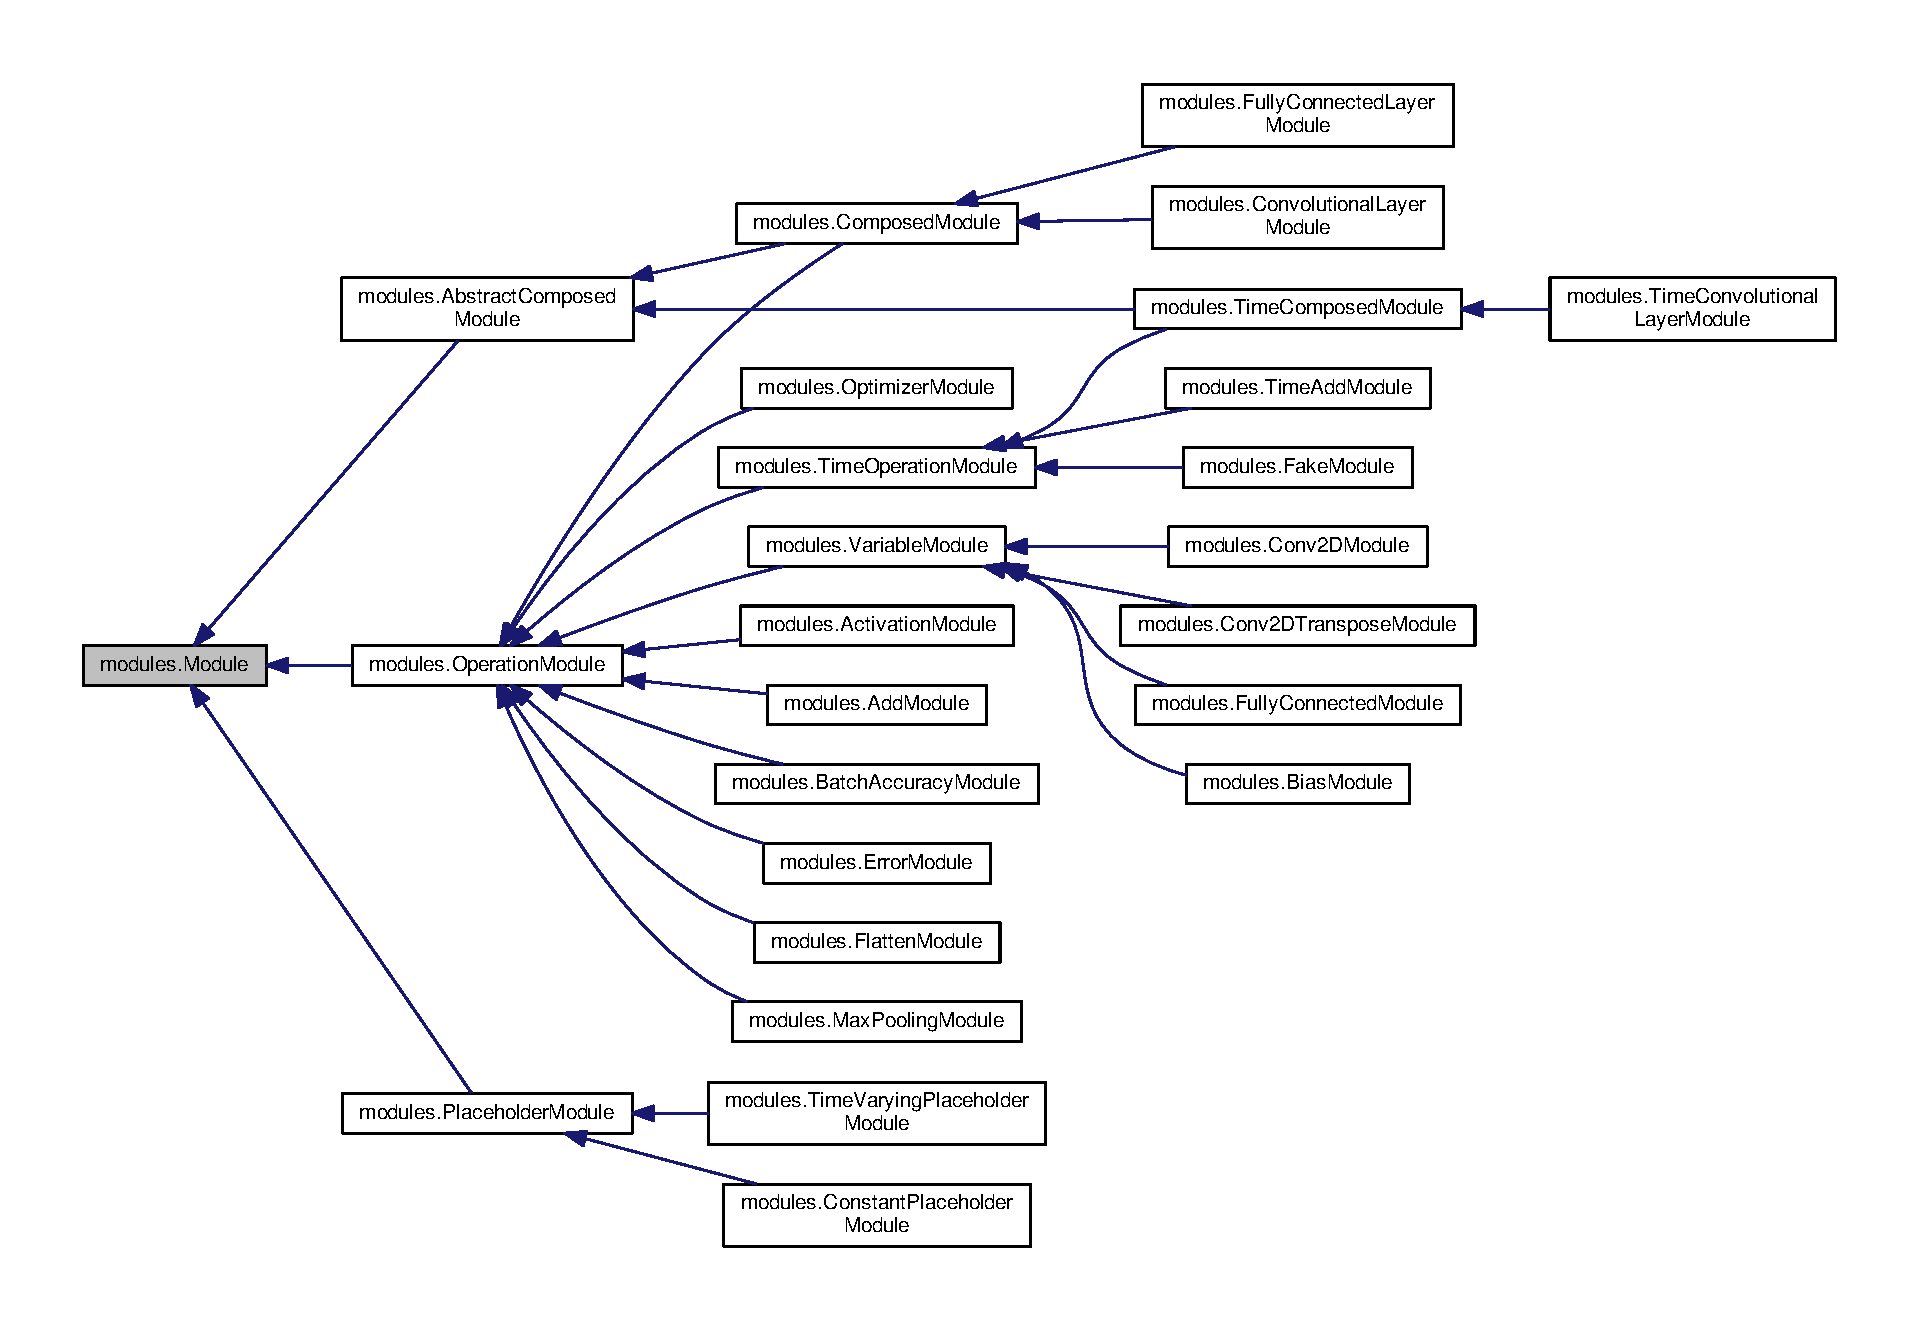
\includegraphics[width=350pt]{classmodules_1_1_module__inherit__graph}
\end{center}
\end{figure}
\subsection*{Public Member Functions}
\begin{DoxyCompactItemize}
\item 
\mbox{\Hypertarget{classmodules_1_1_module_a7811295ea0ad2c9fefd2b205aad7fa29}\label{classmodules_1_1_module_a7811295ea0ad2c9fefd2b205aad7fa29}} 
def {\bfseries \+\_\+\+\_\+init\+\_\+\+\_\+} (self, name, args, kwargs)
\item 
\mbox{\Hypertarget{classmodules_1_1_module_a9a4b685e73bdcaa68764633e93a11935}\label{classmodules_1_1_module_a9a4b685e73bdcaa68764633e93a11935}} 
def {\bfseries output\+\_\+exists} (self, t)
\item 
\mbox{\Hypertarget{classmodules_1_1_module_a5200523b4f6bdc74e06059599546a2a3}\label{classmodules_1_1_module_a5200523b4f6bdc74e06059599546a2a3}} 
def {\bfseries need\+\_\+to\+\_\+create\+\_\+output} (self, t)
\item 
\mbox{\Hypertarget{classmodules_1_1_module_ad0a7fdcec077c92e3f3fdf785ffeea34}\label{classmodules_1_1_module_ad0a7fdcec077c92e3f3fdf785ffeea34}} 
def {\bfseries create\+\_\+output} (self, t)
\item 
\mbox{\Hypertarget{classmodules_1_1_module_a43c6b4fc93a1d339b96fa78f39ab583e}\label{classmodules_1_1_module_a43c6b4fc93a1d339b96fa78f39ab583e}} 
def {\bfseries input\+\_\+tensors} (self, t)
\end{DoxyCompactItemize}
\subsection*{Public Attributes}
\begin{DoxyCompactItemize}
\item 
\mbox{\Hypertarget{classmodules_1_1_module_a37837da834db83c1d452514df6741d64}\label{classmodules_1_1_module_a37837da834db83c1d452514df6741d64}} 
{\bfseries inputs}
\item 
\mbox{\Hypertarget{classmodules_1_1_module_a3d68775d21b0007ffb804db208e3518e}\label{classmodules_1_1_module_a3d68775d21b0007ffb804db208e3518e}} 
{\bfseries outputs}
\item 
\mbox{\Hypertarget{classmodules_1_1_module_adc4d5e494a9ce5c33c684ae4952a4564}\label{classmodules_1_1_module_adc4d5e494a9ce5c33c684ae4952a4564}} 
{\bfseries name}
\end{DoxyCompactItemize}


\subsection{Detailed Description}
Base class of a module. 


\begin{DoxyParams}{Parameters}
{\em name} & str, every module must have a name \\
\hline
\end{DoxyParams}


The documentation for this class was generated from the following file\+:\begin{DoxyCompactItemize}
\item 
/home/cwilmot/\+Documents/\+F\+I\+A\+S/phd/code/python/modules/src/modules.\+py\end{DoxyCompactItemize}

\hypertarget{classmodules_1_1_operation_module}{}\section{modules.\+Operation\+Module Class Reference}
\label{classmodules_1_1_operation_module}\index{modules.\+Operation\+Module@{modules.\+Operation\+Module}}


An operation module is a module that can perform an operation on the output of an other module in the same time slice.  




Inheritance diagram for modules.\+Operation\+Module\+:\nopagebreak
\begin{figure}[H]
\begin{center}
\leavevmode
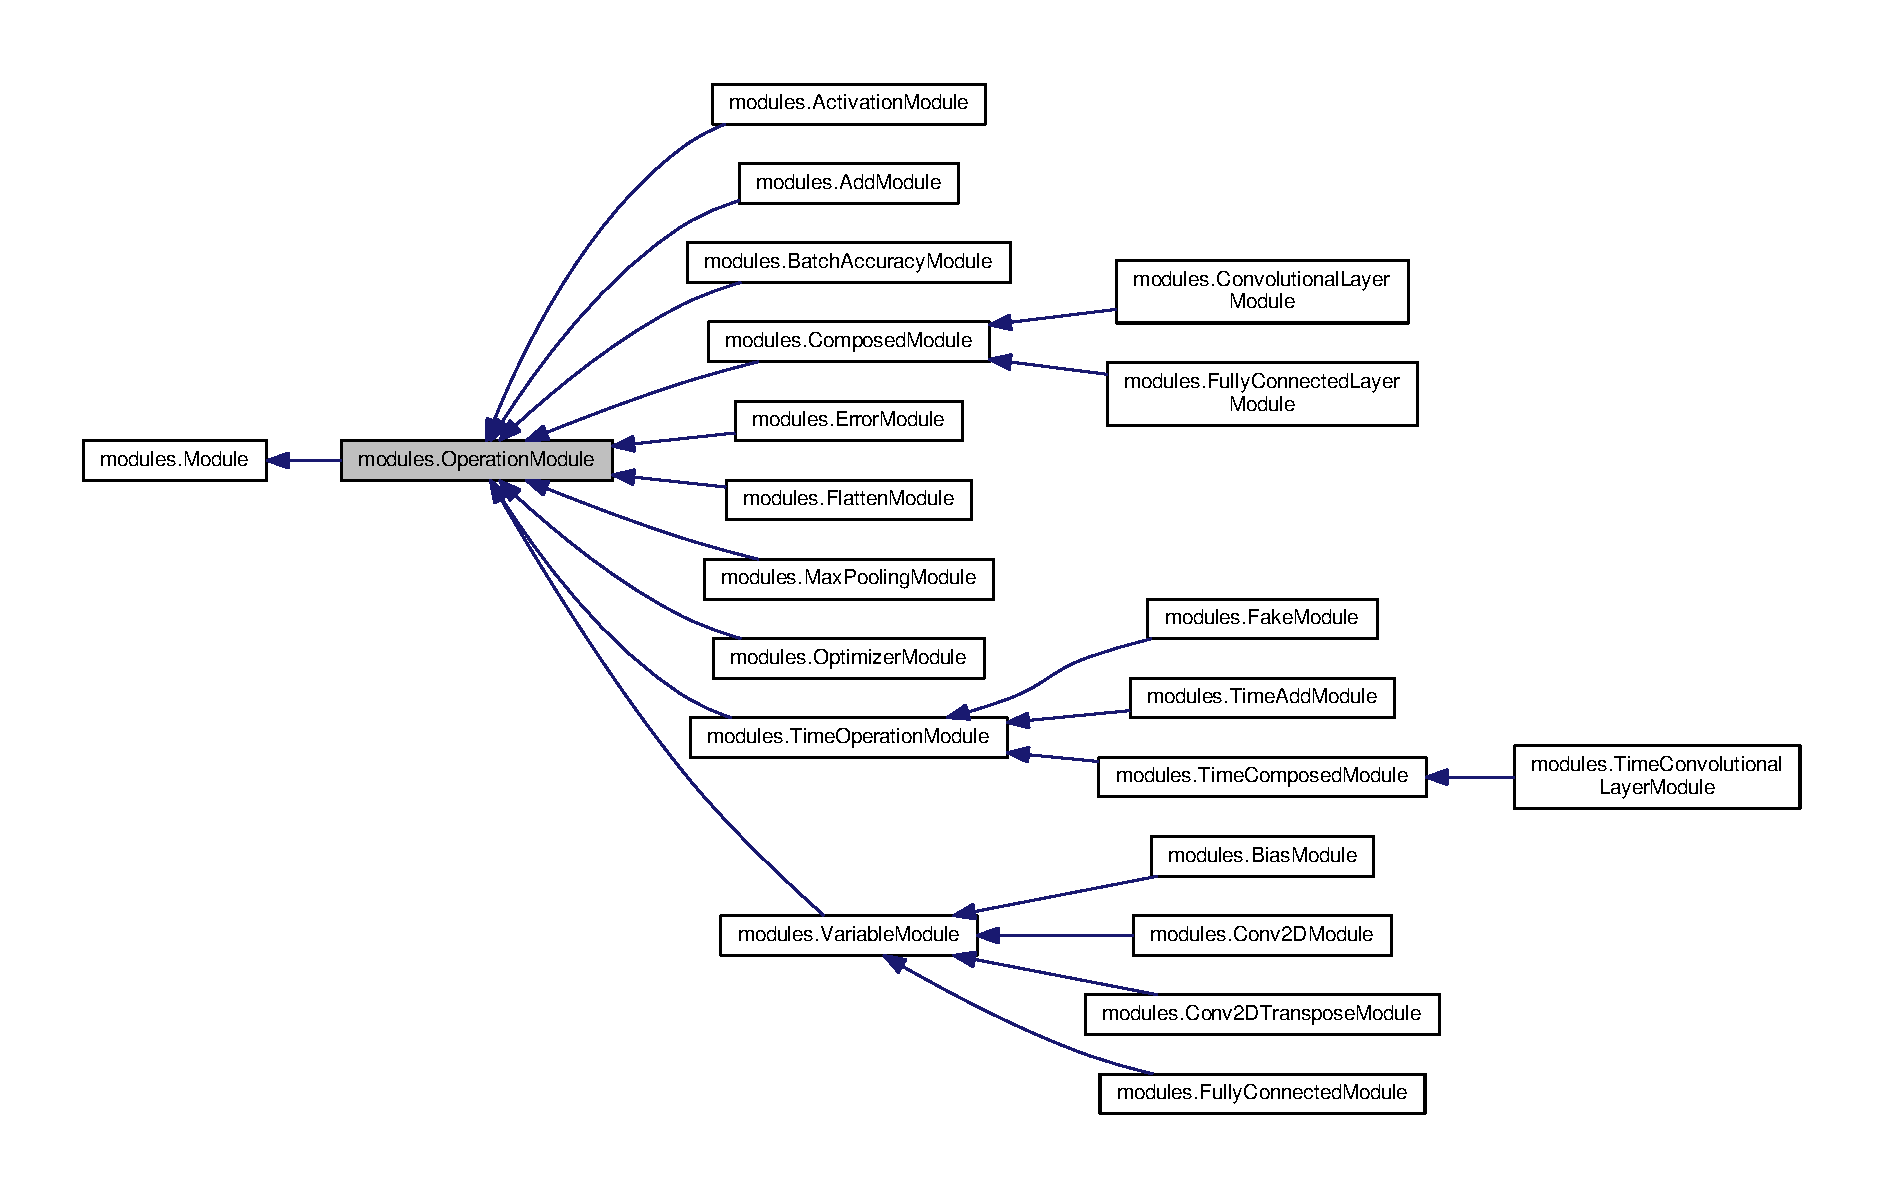
\includegraphics[width=350pt]{classmodules_1_1_operation_module__inherit__graph}
\end{center}
\end{figure}
\subsection*{Public Member Functions}
\begin{DoxyCompactItemize}
\item 
def \hyperlink{classmodules_1_1_operation_module_a781d6ef84166df2f1b08abb324d1f7c8}{add\+\_\+input} (self, other)
\begin{DoxyCompactList}\small\item\em Methode to connect the module to the output of an other module in the same time slice. \end{DoxyCompactList}\item 
\mbox{\Hypertarget{classmodules_1_1_operation_module_ac548115acd3c707e9989ab3cf3ece25b}\label{classmodules_1_1_operation_module_ac548115acd3c707e9989ab3cf3ece25b}} 
def \hyperlink{classmodules_1_1_operation_module_ac548115acd3c707e9989ab3cf3ece25b}{operation} (self, x)
\begin{DoxyCompactList}\small\item\em This methode has to be overwritten. \end{DoxyCompactList}\end{DoxyCompactItemize}
\subsection*{Additional Inherited Members}


\subsection{Detailed Description}
An operation module is a module that can perform an operation on the output of an other module in the same time slice. 

This class is an abstract class. To inherit from it, overwrite the \textquotesingle{}operation\textquotesingle{} methode in the following way\+: the operation methode should take as many parameters as there are modules connected to it and return a tensorflow tensor. These parameters are the output tensors of the previous modules in the same time slice. See the implementation of child classes for more information 

\subsection{Member Function Documentation}
\mbox{\Hypertarget{classmodules_1_1_operation_module_a781d6ef84166df2f1b08abb324d1f7c8}\label{classmodules_1_1_operation_module_a781d6ef84166df2f1b08abb324d1f7c8}} 
\index{modules\+::\+Operation\+Module@{modules\+::\+Operation\+Module}!add\+\_\+input@{add\+\_\+input}}
\index{add\+\_\+input@{add\+\_\+input}!modules\+::\+Operation\+Module@{modules\+::\+Operation\+Module}}
\subsubsection{\texorpdfstring{add\+\_\+input()}{add\_input()}}
{\footnotesize\ttfamily def modules.\+Operation\+Module.\+add\+\_\+input (\begin{DoxyParamCaption}\item[{}]{self,  }\item[{}]{other }\end{DoxyParamCaption})}



Methode to connect the module to the output of an other module in the same time slice. 

mw\+\_\+module.\+add\+\_\+input(other\+\_\+module) 

The documentation for this class was generated from the following file\+:\begin{DoxyCompactItemize}
\item 
/home/cwilmot/\+Documents/\+F\+I\+A\+S/phd/code/python/modules/src/modules.\+py\end{DoxyCompactItemize}

\hypertarget{classmodules_1_1_optimizer_module}{}\section{modules.\+Optimizer\+Module Class Reference}
\label{classmodules_1_1_optimizer_module}\index{modules.\+Optimizer\+Module@{modules.\+Optimizer\+Module}}


\hyperlink{classmodules_1_1_module}{Module} to train a network.  




Inheritance diagram for modules.\+Optimizer\+Module\+:\nopagebreak
\begin{figure}[H]
\begin{center}
\leavevmode
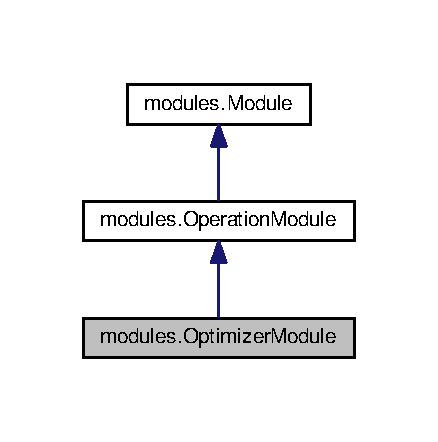
\includegraphics[width=210pt]{classmodules_1_1_optimizer_module__inherit__graph}
\end{center}
\end{figure}
\subsection*{Public Member Functions}
\begin{DoxyCompactItemize}
\item 
def \hyperlink{classmodules_1_1_optimizer_module_a82007e9145e1e80e6485c2de0f7ec5b6}{\+\_\+\+\_\+init\+\_\+\+\_\+} (self, name, optimizer)
\item 
def \hyperlink{classmodules_1_1_optimizer_module_ad8ab7a66f2eb4b2480bd1eea28a28f79}{operation} (self, x)
\begin{DoxyCompactList}\small\item\em returns the output of the input module after adding a dependency in the tensorflow graph. \end{DoxyCompactList}\end{DoxyCompactItemize}
\subsection*{Public Attributes}
\begin{DoxyCompactItemize}
\item 
\mbox{\Hypertarget{classmodules_1_1_optimizer_module_a35feb31fdf5fb6ab303cffe97daa7683}\label{classmodules_1_1_optimizer_module_a35feb31fdf5fb6ab303cffe97daa7683}} 
{\bfseries optimizer}
\end{DoxyCompactItemize}


\subsection{Detailed Description}
\hyperlink{classmodules_1_1_module}{Module} to train a network. 

This module takes a single input module. 

\subsection{Constructor \& Destructor Documentation}
\mbox{\Hypertarget{classmodules_1_1_optimizer_module_a82007e9145e1e80e6485c2de0f7ec5b6}\label{classmodules_1_1_optimizer_module_a82007e9145e1e80e6485c2de0f7ec5b6}} 
\index{modules\+::\+Optimizer\+Module@{modules\+::\+Optimizer\+Module}!\+\_\+\+\_\+init\+\_\+\+\_\+@{\+\_\+\+\_\+init\+\_\+\+\_\+}}
\index{\+\_\+\+\_\+init\+\_\+\+\_\+@{\+\_\+\+\_\+init\+\_\+\+\_\+}!modules\+::\+Optimizer\+Module@{modules\+::\+Optimizer\+Module}}
\subsubsection{\texorpdfstring{\+\_\+\+\_\+init\+\_\+\+\_\+()}{\_\_init\_\_()}}
{\footnotesize\ttfamily def modules.\+Optimizer\+Module.\+\_\+\+\_\+init\+\_\+\+\_\+ (\begin{DoxyParamCaption}\item[{}]{self,  }\item[{}]{name,  }\item[{}]{optimizer }\end{DoxyParamCaption})}


\begin{DoxyParams}{Parameters}
{\em optimizer} & tf.\+train.\+Optimizer, an instance of an optimizer \\
\hline
\end{DoxyParams}


\subsection{Member Function Documentation}
\mbox{\Hypertarget{classmodules_1_1_optimizer_module_ad8ab7a66f2eb4b2480bd1eea28a28f79}\label{classmodules_1_1_optimizer_module_ad8ab7a66f2eb4b2480bd1eea28a28f79}} 
\index{modules\+::\+Optimizer\+Module@{modules\+::\+Optimizer\+Module}!operation@{operation}}
\index{operation@{operation}!modules\+::\+Optimizer\+Module@{modules\+::\+Optimizer\+Module}}
\subsubsection{\texorpdfstring{operation()}{operation()}}
{\footnotesize\ttfamily def modules.\+Optimizer\+Module.\+operation (\begin{DoxyParamCaption}\item[{}]{self,  }\item[{}]{x }\end{DoxyParamCaption})}



returns the output of the input module after adding a dependency in the tensorflow graph. 

Once the output of this module is computed the network is trained 

The documentation for this class was generated from the following file\+:\begin{DoxyCompactItemize}
\item 
/home/cwilmot/\+Documents/\+F\+I\+A\+S/phd/code/python/modules/src/modules.\+py\end{DoxyCompactItemize}

\hypertarget{classmodules_1_1_placeholder_module}{}\section{modules.\+Placeholder\+Module Class Reference}
\label{classmodules_1_1_placeholder_module}\index{modules.\+Placeholder\+Module@{modules.\+Placeholder\+Module}}


A placeholder module is a module that takes no input.  




Inheritance diagram for modules.\+Placeholder\+Module\+:\nopagebreak
\begin{figure}[H]
\begin{center}
\leavevmode
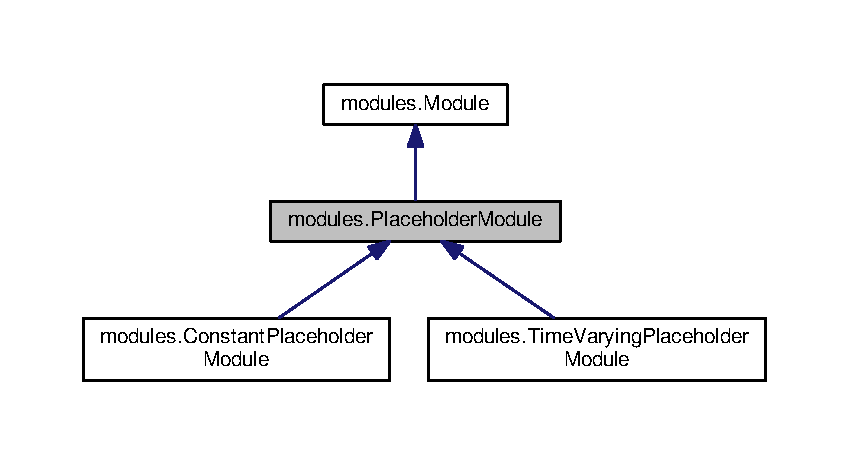
\includegraphics[width=350pt]{classmodules_1_1_placeholder_module__inherit__graph}
\end{center}
\end{figure}
\subsection*{Public Member Functions}
\begin{DoxyCompactItemize}
\item 
\mbox{\Hypertarget{classmodules_1_1_placeholder_module_ac715f9bd0c880b5807baf2954b2e3016}\label{classmodules_1_1_placeholder_module_ac715f9bd0c880b5807baf2954b2e3016}} 
def {\bfseries \+\_\+\+\_\+init\+\_\+\+\_\+} (self, name, shape, dtype=tf.\+float32)
\end{DoxyCompactItemize}
\subsection*{Public Attributes}
\begin{DoxyCompactItemize}
\item 
\mbox{\Hypertarget{classmodules_1_1_placeholder_module_accdf8998b6179f359f4418953fe6a1ea}\label{classmodules_1_1_placeholder_module_accdf8998b6179f359f4418953fe6a1ea}} 
{\bfseries shape}
\item 
\mbox{\Hypertarget{classmodules_1_1_placeholder_module_afd076530b0b38cd09e323c0956275d49}\label{classmodules_1_1_placeholder_module_afd076530b0b38cd09e323c0956275d49}} 
{\bfseries dtype}
\item 
\mbox{\Hypertarget{classmodules_1_1_placeholder_module_a09945c3984e04b0ee2bcdc5cdecfded7}\label{classmodules_1_1_placeholder_module_a09945c3984e04b0ee2bcdc5cdecfded7}} 
{\bfseries placeholder}
\end{DoxyCompactItemize}


\subsection{Detailed Description}
A placeholder module is a module that takes no input. 

It holds a place where the user can feed in a value to be computed in the graph 

The documentation for this class was generated from the following file\+:\begin{DoxyCompactItemize}
\item 
/home/cwilmot/\+Documents/\+F\+I\+A\+S/phd/code/python/modules/src/modules.\+py\end{DoxyCompactItemize}

\hypertarget{classmodules_1_1_time_add_module}{}\section{modules.\+Time\+Add\+Module Class Reference}
\label{classmodules_1_1_time_add_module}\index{modules.\+Time\+Add\+Module@{modules.\+Time\+Add\+Module}}


This module computes the sum of all its input.  




Inheritance diagram for modules.\+Time\+Add\+Module\+:\nopagebreak
\begin{figure}[H]
\begin{center}
\leavevmode
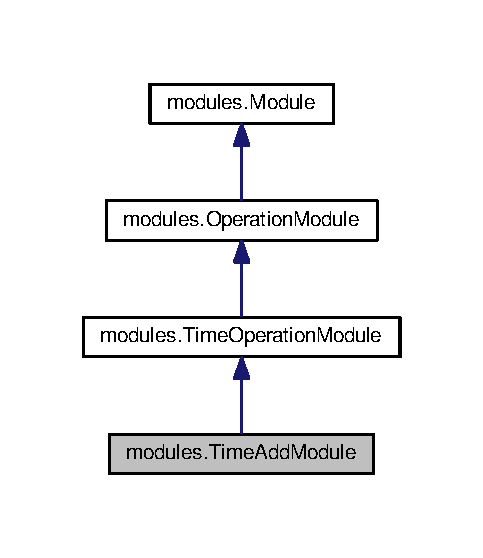
\includegraphics[width=232pt]{classmodules_1_1_time_add_module__inherit__graph}
\end{center}
\end{figure}
\subsection*{Public Member Functions}
\begin{DoxyCompactItemize}
\item 
\mbox{\Hypertarget{classmodules_1_1_time_add_module_a85acb5bdfffdc3a65cbcef78d022310f}\label{classmodules_1_1_time_add_module_a85acb5bdfffdc3a65cbcef78d022310f}} 
def \hyperlink{classmodules_1_1_time_add_module_a85acb5bdfffdc3a65cbcef78d022310f}{operation} (self, args)
\begin{DoxyCompactList}\small\item\em returns the sum of the output tensors of all its input modules \end{DoxyCompactList}\end{DoxyCompactItemize}
\subsection*{Additional Inherited Members}


\subsection{Detailed Description}
This module computes the sum of all its input. 

It can have as many inputs as requiered and support recursions 

The documentation for this class was generated from the following file\+:\begin{DoxyCompactItemize}
\item 
/home/cwilmot/\+Documents/\+F\+I\+A\+S/phd/code/python/modules/src/modules.\+py\end{DoxyCompactItemize}

\hypertarget{classmodules_1_1_time_composed_module}{}\section{modules.\+Time\+Composed\+Module Class Reference}
\label{classmodules_1_1_time_composed_module}\index{modules.\+Time\+Composed\+Module@{modules.\+Time\+Composed\+Module}}


This class is an abstract class which allows when overwritten to create a module that is composed of other modules and accept recursions See the implementation of \hyperlink{classmodules_1_1_convolutional_layer_module}{Convolutional\+Layer\+Module} for more info.  




Inheritance diagram for modules.\+Time\+Composed\+Module\+:\nopagebreak
\begin{figure}[H]
\begin{center}
\leavevmode
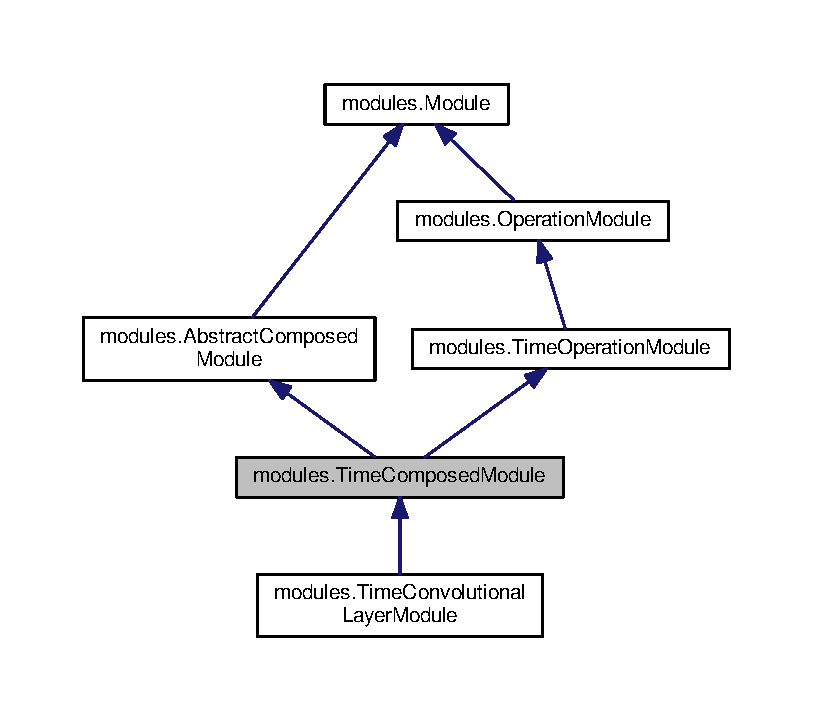
\includegraphics[width=350pt]{classmodules_1_1_time_composed_module__inherit__graph}
\end{center}
\end{figure}
\subsection*{Additional Inherited Members}


\subsection{Detailed Description}
This class is an abstract class which allows when overwritten to create a module that is composed of other modules and accept recursions See the implementation of \hyperlink{classmodules_1_1_convolutional_layer_module}{Convolutional\+Layer\+Module} for more info. 

the methode \textquotesingle{}define\+\_\+inner\+\_\+modules\textquotesingle{} must be overwritten, the attribute input\+\_\+module must be set to the module which is the input of the composed module the attribute output\+\_\+module must be set to the module which is the output of the composed module 

The documentation for this class was generated from the following file\+:\begin{DoxyCompactItemize}
\item 
/home/cwilmot/\+Documents/\+F\+I\+A\+S/phd/code/python/modules/src/modules.\+py\end{DoxyCompactItemize}

\hypertarget{classmodules_1_1_time_convolutional_layer_module}{}\section{modules.\+Time\+Convolutional\+Layer\+Module Class Reference}
\label{classmodules_1_1_time_convolutional_layer_module}\index{modules.\+Time\+Convolutional\+Layer\+Module@{modules.\+Time\+Convolutional\+Layer\+Module}}


This composed module performs a convolution and applies a bias and an activation function.  




Inheritance diagram for modules.\+Time\+Convolutional\+Layer\+Module\+:\nopagebreak
\begin{figure}[H]
\begin{center}
\leavevmode
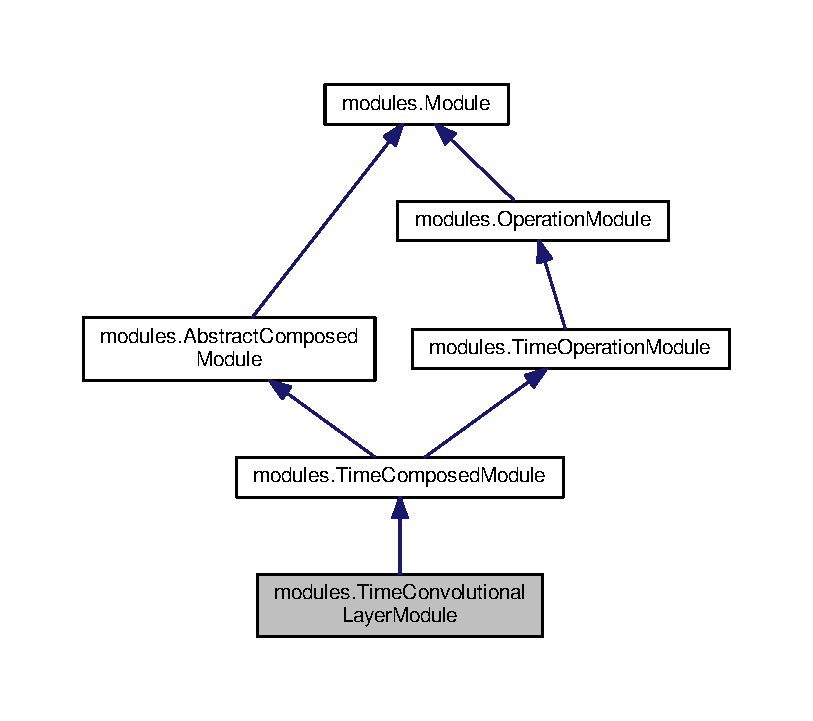
\includegraphics[width=350pt]{classmodules_1_1_time_convolutional_layer_module__inherit__graph}
\end{center}
\end{figure}
\subsection*{Public Member Functions}
\begin{DoxyCompactItemize}
\item 
\mbox{\Hypertarget{classmodules_1_1_time_convolutional_layer_module_abd09adc52e8ba14364ade4f8196e4fcb}\label{classmodules_1_1_time_convolutional_layer_module_abd09adc52e8ba14364ade4f8196e4fcb}} 
def {\bfseries define\+\_\+inner\+\_\+modules} (self, name, activation, filter\+\_\+shape, strides, bias\+\_\+shape, padding=\textquotesingle{}S\+A\+ME\textquotesingle{})
\end{DoxyCompactItemize}
\subsection*{Public Attributes}
\begin{DoxyCompactItemize}
\item 
\mbox{\Hypertarget{classmodules_1_1_time_convolutional_layer_module_ae677272a2f73e35433150f011bcc4338}\label{classmodules_1_1_time_convolutional_layer_module_ae677272a2f73e35433150f011bcc4338}} 
{\bfseries input\+\_\+module}
\item 
\mbox{\Hypertarget{classmodules_1_1_time_convolutional_layer_module_a1bedce8250b63fb0b1987279947da8f2}\label{classmodules_1_1_time_convolutional_layer_module_a1bedce8250b63fb0b1987279947da8f2}} 
{\bfseries conv}
\item 
\mbox{\Hypertarget{classmodules_1_1_time_convolutional_layer_module_a96caa16034d47b22cb8af83339c0e0bb}\label{classmodules_1_1_time_convolutional_layer_module_a96caa16034d47b22cb8af83339c0e0bb}} 
{\bfseries bias}
\item 
\mbox{\Hypertarget{classmodules_1_1_time_convolutional_layer_module_aa3826156422a0d3c52cf81c2a7500b6e}\label{classmodules_1_1_time_convolutional_layer_module_aa3826156422a0d3c52cf81c2a7500b6e}} 
{\bfseries preactivation}
\item 
\mbox{\Hypertarget{classmodules_1_1_time_convolutional_layer_module_a822d0c075c48bae8208648ae3bbf49ff}\label{classmodules_1_1_time_convolutional_layer_module_a822d0c075c48bae8208648ae3bbf49ff}} 
{\bfseries output\+\_\+module}
\end{DoxyCompactItemize}


\subsection{Detailed Description}
This composed module performs a convolution and applies a bias and an activation function. 

It does allow recursions 

The documentation for this class was generated from the following file\+:\begin{DoxyCompactItemize}
\item 
/home/cwilmot/\+Documents/\+F\+I\+A\+S/phd/code/python/modules/src/modules.\+py\end{DoxyCompactItemize}

\hypertarget{classmodules_1_1_time_operation_module}{}\section{modules.\+Time\+Operation\+Module Class Reference}
\label{classmodules_1_1_time_operation_module}\index{modules.\+Time\+Operation\+Module@{modules.\+Time\+Operation\+Module}}


Same as an \hyperlink{classmodules_1_1_operation_module}{Operation\+Module} but this class allows to connect itself with the output of an other module in a different time slice.  




Inheritance diagram for modules.\+Time\+Operation\+Module\+:\nopagebreak
\begin{figure}[H]
\begin{center}
\leavevmode
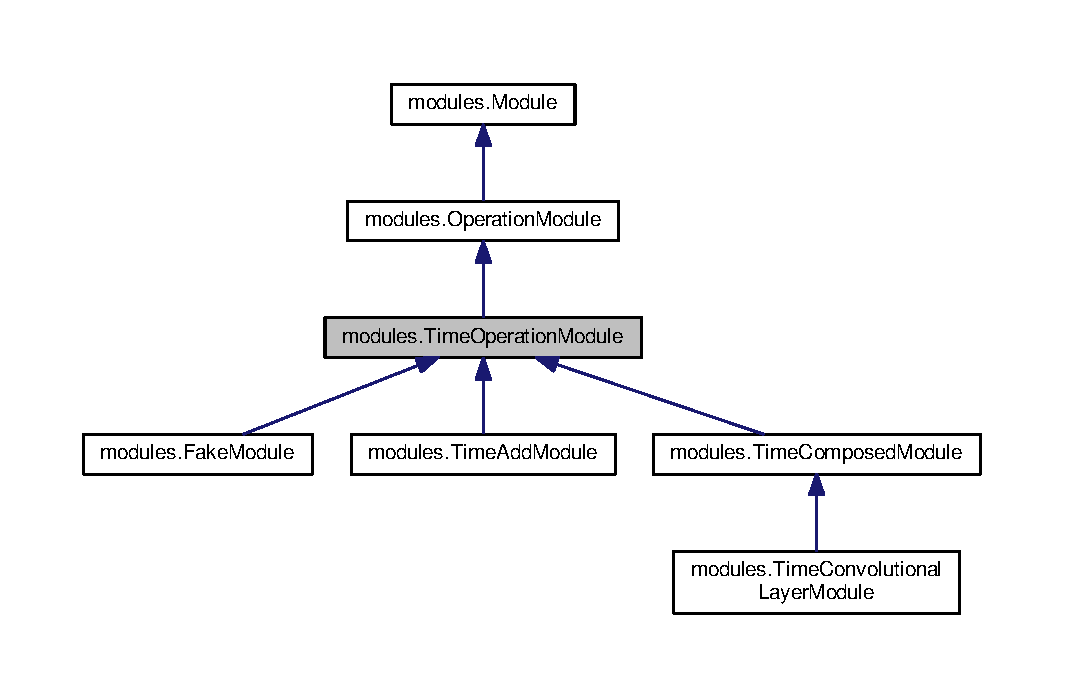
\includegraphics[width=350pt]{classmodules_1_1_time_operation_module__inherit__graph}
\end{center}
\end{figure}
\subsection*{Public Member Functions}
\begin{DoxyCompactItemize}
\item 
def \hyperlink{classmodules_1_1_time_operation_module_a3076a344fba6d85b134a6d4b5d2fba46}{add\+\_\+input} (self, other, t)
\begin{DoxyCompactList}\small\item\em Methode to connect the module to the output of an other module in the same OR AN O\+T\+H\+ER time slice. \end{DoxyCompactList}\end{DoxyCompactItemize}
\subsection*{Additional Inherited Members}


\subsection{Detailed Description}
Same as an \hyperlink{classmodules_1_1_operation_module}{Operation\+Module} but this class allows to connect itself with the output of an other module in a different time slice. 

Those two kinds of modules are separated to help the developer to keep the connectivity of his modules clear. 

\subsection{Member Function Documentation}
\mbox{\Hypertarget{classmodules_1_1_time_operation_module_a3076a344fba6d85b134a6d4b5d2fba46}\label{classmodules_1_1_time_operation_module_a3076a344fba6d85b134a6d4b5d2fba46}} 
\index{modules\+::\+Time\+Operation\+Module@{modules\+::\+Time\+Operation\+Module}!add\+\_\+input@{add\+\_\+input}}
\index{add\+\_\+input@{add\+\_\+input}!modules\+::\+Time\+Operation\+Module@{modules\+::\+Time\+Operation\+Module}}
\subsubsection{\texorpdfstring{add\+\_\+input()}{add\_input()}}
{\footnotesize\ttfamily def modules.\+Time\+Operation\+Module.\+add\+\_\+input (\begin{DoxyParamCaption}\item[{}]{self,  }\item[{}]{other,  }\item[{}]{t }\end{DoxyParamCaption})}



Methode to connect the module to the output of an other module in the same OR AN O\+T\+H\+ER time slice. 

mw\+\_\+module.\+add\+\_\+input(other\+\_\+module,  0) \# same time slice mw\+\_\+module.\+add\+\_\+input(other\+\_\+module, -\/1) \# previous time slice connecting the module to a future time slice (ie t=1, 2...) makes no sens 
\begin{DoxyParams}{Parameters}
{\em other} & \hyperlink{classmodules_1_1_module}{Module}, an other module \\
\hline
{\em t} & int, the delta t which specify to which time slice to connect to \\
\hline
\end{DoxyParams}


The documentation for this class was generated from the following file\+:\begin{DoxyCompactItemize}
\item 
/home/cwilmot/\+Documents/\+F\+I\+A\+S/phd/code/python/modules/src/modules.\+py\end{DoxyCompactItemize}

\hypertarget{classmodules_1_1_time_varying_placeholder_module}{}\section{modules.\+Time\+Varying\+Placeholder\+Module Class Reference}
\label{classmodules_1_1_time_varying_placeholder_module}\index{modules.\+Time\+Varying\+Placeholder\+Module@{modules.\+Time\+Varying\+Placeholder\+Module}}


\hyperlink{classmodules_1_1_module}{Module} to reserve a place to feed in data.  




Inheritance diagram for modules.\+Time\+Varying\+Placeholder\+Module\+:\nopagebreak
\begin{figure}[H]
\begin{center}
\leavevmode
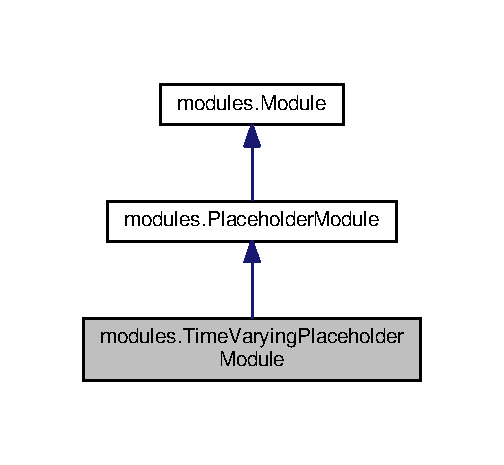
\includegraphics[width=242pt]{classmodules_1_1_time_varying_placeholder_module__inherit__graph}
\end{center}
\end{figure}
\subsection*{Public Member Functions}
\begin{DoxyCompactItemize}
\item 
\mbox{\Hypertarget{classmodules_1_1_time_varying_placeholder_module_aabf6878d8bd17b00fbdbe1e0a8fe9c0a}\label{classmodules_1_1_time_varying_placeholder_module_aabf6878d8bd17b00fbdbe1e0a8fe9c0a}} 
def {\bfseries \+\_\+\+\_\+init\+\_\+\+\_\+} (self, name, shape, dtype=tf.\+float32)
\item 
\mbox{\Hypertarget{classmodules_1_1_time_varying_placeholder_module_ac6514ecbe9d187d657fc86c071e2e756}\label{classmodules_1_1_time_varying_placeholder_module_ac6514ecbe9d187d657fc86c071e2e756}} 
def {\bfseries get\+\_\+max\+\_\+time} (self)
\item 
\mbox{\Hypertarget{classmodules_1_1_time_varying_placeholder_module_a432646952b2df102f5da026f66addf7c}\label{classmodules_1_1_time_varying_placeholder_module_a432646952b2df102f5da026f66addf7c}} 
def {\bfseries need\+\_\+to\+\_\+create\+\_\+output} (self, t)
\item 
\mbox{\Hypertarget{classmodules_1_1_time_varying_placeholder_module_a4e07fcf5b491485a38fa42dd9e2fc8c7}\label{classmodules_1_1_time_varying_placeholder_module_a4e07fcf5b491485a38fa42dd9e2fc8c7}} 
def {\bfseries shift\+\_\+by\+\_\+one} (self)
\item 
\mbox{\Hypertarget{classmodules_1_1_time_varying_placeholder_module_a8c97b431ed39651472ff304b03e04036}\label{classmodules_1_1_time_varying_placeholder_module_a8c97b431ed39651472ff304b03e04036}} 
def {\bfseries delayed} (self, v)
\item 
\mbox{\Hypertarget{classmodules_1_1_time_varying_placeholder_module_a26a9bfa037aae7d52b975e27e1476ccc}\label{classmodules_1_1_time_varying_placeholder_module_a26a9bfa037aae7d52b975e27e1476ccc}} 
def {\bfseries create\+\_\+output} (self, t)
\end{DoxyCompactItemize}
\subsection*{Properties}
\begin{DoxyCompactItemize}
\item 
\mbox{\Hypertarget{classmodules_1_1_time_varying_placeholder_module_af20479b3474a90c46f4bde69f2f07271}\label{classmodules_1_1_time_varying_placeholder_module_af20479b3474a90c46f4bde69f2f07271}} 
{\bfseries max\+\_\+time} = property(get\+\_\+max\+\_\+time)
\end{DoxyCompactItemize}
\subsection*{Additional Inherited Members}


\subsection{Detailed Description}
\hyperlink{classmodules_1_1_module}{Module} to reserve a place to feed in data. 

It remembers the input wich is fed by the user and roll it so that at each time slice the network sees a new value. This module takes no input. 

The documentation for this class was generated from the following file\+:\begin{DoxyCompactItemize}
\item 
/home/cwilmot/\+Documents/\+F\+I\+A\+S/phd/code/python/modules/src/modules.\+py\end{DoxyCompactItemize}

\hypertarget{classmodules_1_1_variable_module}{}\section{modules.\+Variable\+Module Class Reference}
\label{classmodules_1_1_variable_module}\index{modules.\+Variable\+Module@{modules.\+Variable\+Module}}


This class allows a module to hold a tensorflow variable.  




Inheritance diagram for modules.\+Variable\+Module\+:\nopagebreak
\begin{figure}[H]
\begin{center}
\leavevmode
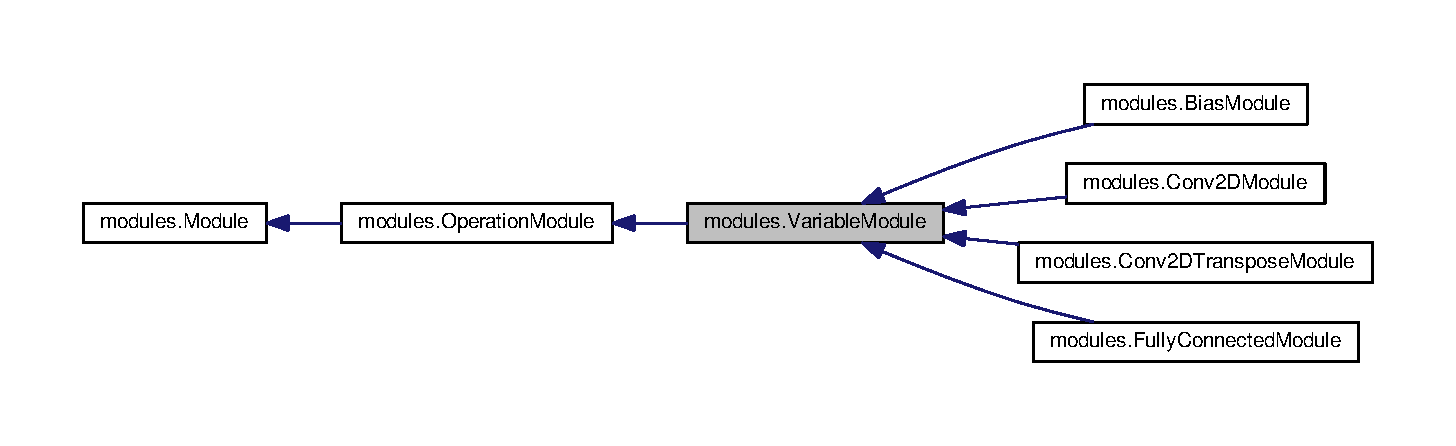
\includegraphics[width=350pt]{classmodules_1_1_variable_module__inherit__graph}
\end{center}
\end{figure}
\subsection*{Public Member Functions}
\begin{DoxyCompactItemize}
\item 
\mbox{\Hypertarget{classmodules_1_1_variable_module_a01b71eae9cc4d56107269d110a5a41c4}\label{classmodules_1_1_variable_module_a01b71eae9cc4d56107269d110a5a41c4}} 
def {\bfseries \+\_\+\+\_\+init\+\_\+\+\_\+} (self, args, kwargs)
\item 
def \hyperlink{classmodules_1_1_variable_module_a7a01e27208c41122163147ff0cf73fe8}{create\+\_\+variables} (self, name)
\begin{DoxyCompactList}\small\item\em Methode to create tensorflow variables. \end{DoxyCompactList}\end{DoxyCompactItemize}
\subsection*{Additional Inherited Members}


\subsection{Detailed Description}
This class allows a module to hold a tensorflow variable. 

To do so, you have to overwrite the \textquotesingle{}create\+\_\+variables\textquotesingle{} methode. It is then automatically called by the constructor. See child classes for more details. 

\subsection{Member Function Documentation}
\mbox{\Hypertarget{classmodules_1_1_variable_module_a7a01e27208c41122163147ff0cf73fe8}\label{classmodules_1_1_variable_module_a7a01e27208c41122163147ff0cf73fe8}} 
\index{modules\+::\+Variable\+Module@{modules\+::\+Variable\+Module}!create\+\_\+variables@{create\+\_\+variables}}
\index{create\+\_\+variables@{create\+\_\+variables}!modules\+::\+Variable\+Module@{modules\+::\+Variable\+Module}}
\subsubsection{\texorpdfstring{create\+\_\+variables()}{create\_variables()}}
{\footnotesize\ttfamily def modules.\+Variable\+Module.\+create\+\_\+variables (\begin{DoxyParamCaption}\item[{}]{self,  }\item[{}]{name }\end{DoxyParamCaption})}



Methode to create tensorflow variables. 

This methode must be overwritten 
\begin{DoxyParams}{Parameters}
{\em name} & str, implementation must be changed, the name can be accessed from self \\
\hline
\end{DoxyParams}


The documentation for this class was generated from the following file\+:\begin{DoxyCompactItemize}
\item 
/home/cwilmot/\+Documents/\+F\+I\+A\+S/phd/code/python/modules/src/modules.\+py\end{DoxyCompactItemize}

%--- End generated contents ---

% Index
\backmatter
\newpage
\phantomsection
\clearemptydoublepage
\addcontentsline{toc}{chapter}{Index}
\printindex

\end{document}
